% Paquets généraux
\documentclass[a4paper,12pt,titlepage]{article}
\usepackage[T1]{fontenc}
\usepackage[utf8]{inputenc}
\usepackage[french]{babel}
\usepackage[gen]{eurosym}
%\usepackage[dvips]{graphicx}
\usepackage{fancyhdr}
\usepackage{pdfpages} 
\usepackage{multido}
\usepackage{hyperref}
%\usepackage{textcomp}
%\usepackage{aeguill}
\usepackage{schemabloc}
\usepackage[bitstream-charter]{mathdesign}

\newcommand{\id}{54}
\newcommand{\nom}{Liaisons mécaniques}
\newcommand{\sequence}{04}
\newcommand{\num}{01}
\newcommand{\type}{TP}
\newcommand{\descrip}{Modélisation d'un solide. Comportement des liaisons mécaniques. Modéliser les mécanismes du laboratoire par un schéma cinématique, paramétré.}
\newcommand{\competences}{A3-C4: Analyse d'architecture et de comportement \\ &  Mod1-C1: Isolement d'un solide ou d'un système de solides \\ &  Mod2-C10-1: Modèle de solide indéformable \\ &  Mod2-C11: Modélisation géométrique et cinématique des mouvements entre solides indéformables \\ &  Mod2-C12: Modélisation cinématique des liaisons entre solides \\ &  Mod2-C15: Modélisation des actions mécaniques \\ &  Rés-C6: Utilisation d'un solveur ou d'un logiciel multi physique \\ &  Com1-C1: Différents descripteurs introduits dans le programme \\ &  Com2-C4: Outils de communication}
\newcommand{\nbcomp}{9}
\newcommand{\systemes}{Plateforme Stewart}
\newcommand{\systemessansaccent}{Plateforme Stewart}
\newcommand{\ilot}{2}
\newcommand{\ilotstr}{02}
\newcommand{\dossierilot}{\detokenize{Ilot_02 Plateforme Stewart}}
\newcommand{\imageun}{Plateforme}

\newcommand{\urlsysteme}{\href{https://www.costadoat.fr/systeme/57}{Ressources système}}
\newcommand{\matlabsimscape}{\href{https://github.com/Costadoat/Sciences-Ingenieur/raw/master/Systemes/Plateforme Stewart/Plateforme_Stewart_Simscape.zip}{Modèle Simscape}}
\newcommand{\solidworks}{\href{https://github.com/Costadoat/Sciences-Ingenieur/raw/master/Systemes/Plateforme Stewart/Plateforme_Stewart_Solidworks.zip}{Modèle Solidworks}}
\newcommand{\edrawings}{\href{https://github.com/Costadoat/Sciences-Ingenieur/raw/master/Systemes/Plateforme Stewart/Plateforme_Stewart.EASM}{Modèle eDrawings}}
\newcommand{\test}{Stewart_param1}
\newcommand{\testi}{Stewart_param2}
\newcommand{\testii}{Stewart_param3}
\newcommand{\testiii}{Stewart_param4}
\newcommand{\testiiii}{Stewart_euler}

\newcommand{\auteurun}{Renaud Costadoat}
\newcommand{\auteurdeux}{Françoise Puig}
\newcommand{\institute}{Lycée Dorian}


\usepackage{color}
\usepackage{xcolor}
\usepackage{colortbl}
\usepackage{helvet}
\renewcommand{\familydefault}{\sfdefault}
\usepackage{amsfonts}
\usepackage{amsmath}
%\usepackage{xspace}
\usepackage{varioref}
\usepackage{tabularx}
%\usepackage{floatflt}
\usepackage{graphics}
\usepackage{wrapfig}
\usepackage{textcomp}
\usepackage{tikz}
\usepackage{wrapfig}
\usepackage{gensymb}
\usepackage[european]{circuitikz}
\usetikzlibrary{babel}
\usepackage{ifthen}
\usepackage{cancel}
\usepackage{etoolbox}
\usepackage{multirow}
%\usepackage{boxedminipage}
\definecolor{gris25}{gray}{0.75}
\definecolor{bleu}{RGB}{18,33,98}
\definecolor{bleuf}{RGB}{42,94,171}
\definecolor{bleuc}{RGB}{231,239,247}
\definecolor{rougef}{RGB}{185,18,27}
\definecolor{rougec}{RGB}{255,188,204}%255,230,231
\definecolor{vertf}{RGB}{103,126,82}
\definecolor{vertc}{RGB}{220,255,191}
\definecolor{forestgreen}{rgb}{0.13,0.54,0.13}
\definecolor{blcr}{rgb}{0.59,0.69,0.84}
\definecolor{blfr}{rgb}{0.32,0.51,0.75}
\definecolor{orfr}{rgb}{0.90,0.42,0.15}
\definecolor{orcr}{rgb}{0.90,0.65,0.50}
\definecolor{orangef}{rgb}{0.659,0.269,0.072}
\definecolor{orange}{rgb}{0.58,0.35,0.063}
\definecolor{orangec}{rgb}{0.43,0.32,0.25}
\definecolor{rcorrect}{rgb}{0.6,0,0}
\definecolor{sequence}{rgb}{0.75,0.75,0.75}
\definecolor{competences}{rgb}{0.61,0.73,0.35}
\definecolor{grisf}{HTML}{222222}
\definecolor{grisc}{HTML}{636363}
\definecolor{normal}{HTML}{4087c4}
\definecolor{info}{HTML}{5bc0de}
\definecolor{success}{RGB}{92,184,92}
\definecolor{warning}{RGB}{240,173,78}
\definecolor{danger}{RGB}{217,83,79}
\hypersetup{                    % parametrage des hyperliens
    colorlinks=true,                % colorise les liens
    breaklinks=true,                % permet les retours à la ligne pour les liens trop longs
    urlcolor= blfr,                 % couleur des hyperliens
    linkcolor= orange,                % couleur des liens internes aux documents (index, figures, tableaux, equations,...)
    citecolor= forestgreen                % couleur des liens vers les references bibliographiques
    }

% Mise en page
\pagestyle{fancy}

\setlength{\hoffset}{-18pt}

\setlength{\oddsidemargin}{0pt} 	% Marge gauche sur pages impaires
\setlength{\evensidemargin}{0pt} 	% Marge gauche sur pages paires
\setlength{\marginparwidth}{00pt} 	% Largeur de note dans la marge
\setlength{\headwidth}{481pt} 	 	% Largeur de la zone de tête (17cm)
\setlength{\textwidth}{481pt} 	 	% Largeur de la zone de texte (17cm)
\setlength{\voffset}{-18pt} 		% Bon pour DOS
\setlength{\marginparsep}{7pt}	 	% Séparation de la marge
\setlength{\topmargin}{-30pt} 		% Pas de marge en haut
\setlength{\headheight}{35pt} 		% Haut de page
\setlength{\headsep}{20pt} 		% Entre le haut de page et le texte
\setlength{\footskip}{30pt} 		% Bas de page + séparation
\setlength{\textheight}{700pt} 		% Hauteur de l'icone zone de texte (25cm)
\setlength\fboxrule{1 pt}
\renewcommand{\baselinestretch}{1}
\setcounter{tocdepth}{1}
\newcommand{\cadre}[2]
{\fbox{
  \begin{minipage}{#1\linewidth}
   \begin{center}
    #2\\
   \end{center}
  \end{minipage}
 }
}

\newcounter{num_quest} \setcounter{num_quest}{0}
\newcounter{num_rep} \setcounter{num_rep}{0}
\newcounter{num_cor} \setcounter{num_cor}{0}

\newcommand{\question}[1]{\refstepcounter{num_quest}\par
~\ \\ \parbox[t][][t]{0.15\linewidth}{\textbf{Question \arabic{num_quest}}}\parbox[t][][t]{0.93\linewidth}{#1}\par
}


\newcommand{\reponse}[1]
{\refstepcounter{num_rep}
\noindent
\rule{\linewidth}{.5pt}
\textbf{Question \arabic{num_rep}:}
\multido{\i=1+1}{#1}{~\ \\}
}

\newcommand{\cor}
{\refstepcounter{num_cor}
\noindent
\rule{\linewidth}{.5pt}
\textbf{Question \arabic{num_cor}:} \\
}

\newcommand{\titre}[1]
{\begin{center}
\cadre{0.8}{\huge #1} 
\end{center}
}


% En tête et pied de page
\fancypagestyle{normal}{%
  \fancyhf{}
\lhead{\nom}
\rhead{
\includegraphics[width=2cm]{../../img/logo}\hspace{2pt}}
\ifdef{\auteurdeux}{\lfoot{\auteurun,\auteurdeux}}{\lfoot{\auteurun}}
\cfoot{Page \thepage}}

\fancypagestyle{correction}{%
  \fancyhf{}
  \lhead{\colorbox{danger}{\begin{minipage}{0.65\paperwidth} \textcolor{white}{\textbf{Correction}} \end{minipage}} }
  \rhead{
\includegraphics[width=2cm]{../../img/logo}}
  \ifdef{\auteurdeux}{\lfoot{\auteurun,\auteurdeux}}{\lfoot{\auteurun}}
  \rfoot{\colorbox{danger}{\begin{minipage}{0.5\paperwidth} \begin{flushright}\textcolor{white}{\textbf{Correction}}\end{flushright} \end{minipage}} }}

\renewcommand{\footrulewidth}{0.4pt}

\usepackage{eso-pic}
\newcommand{\BackgroundPic}{%
\put(0,0){%
\parbox[b][\paperheight]{\paperwidth}{%
\vfill
\begin{center}
\hspace{0.5cm}\vspace{0.5cm}
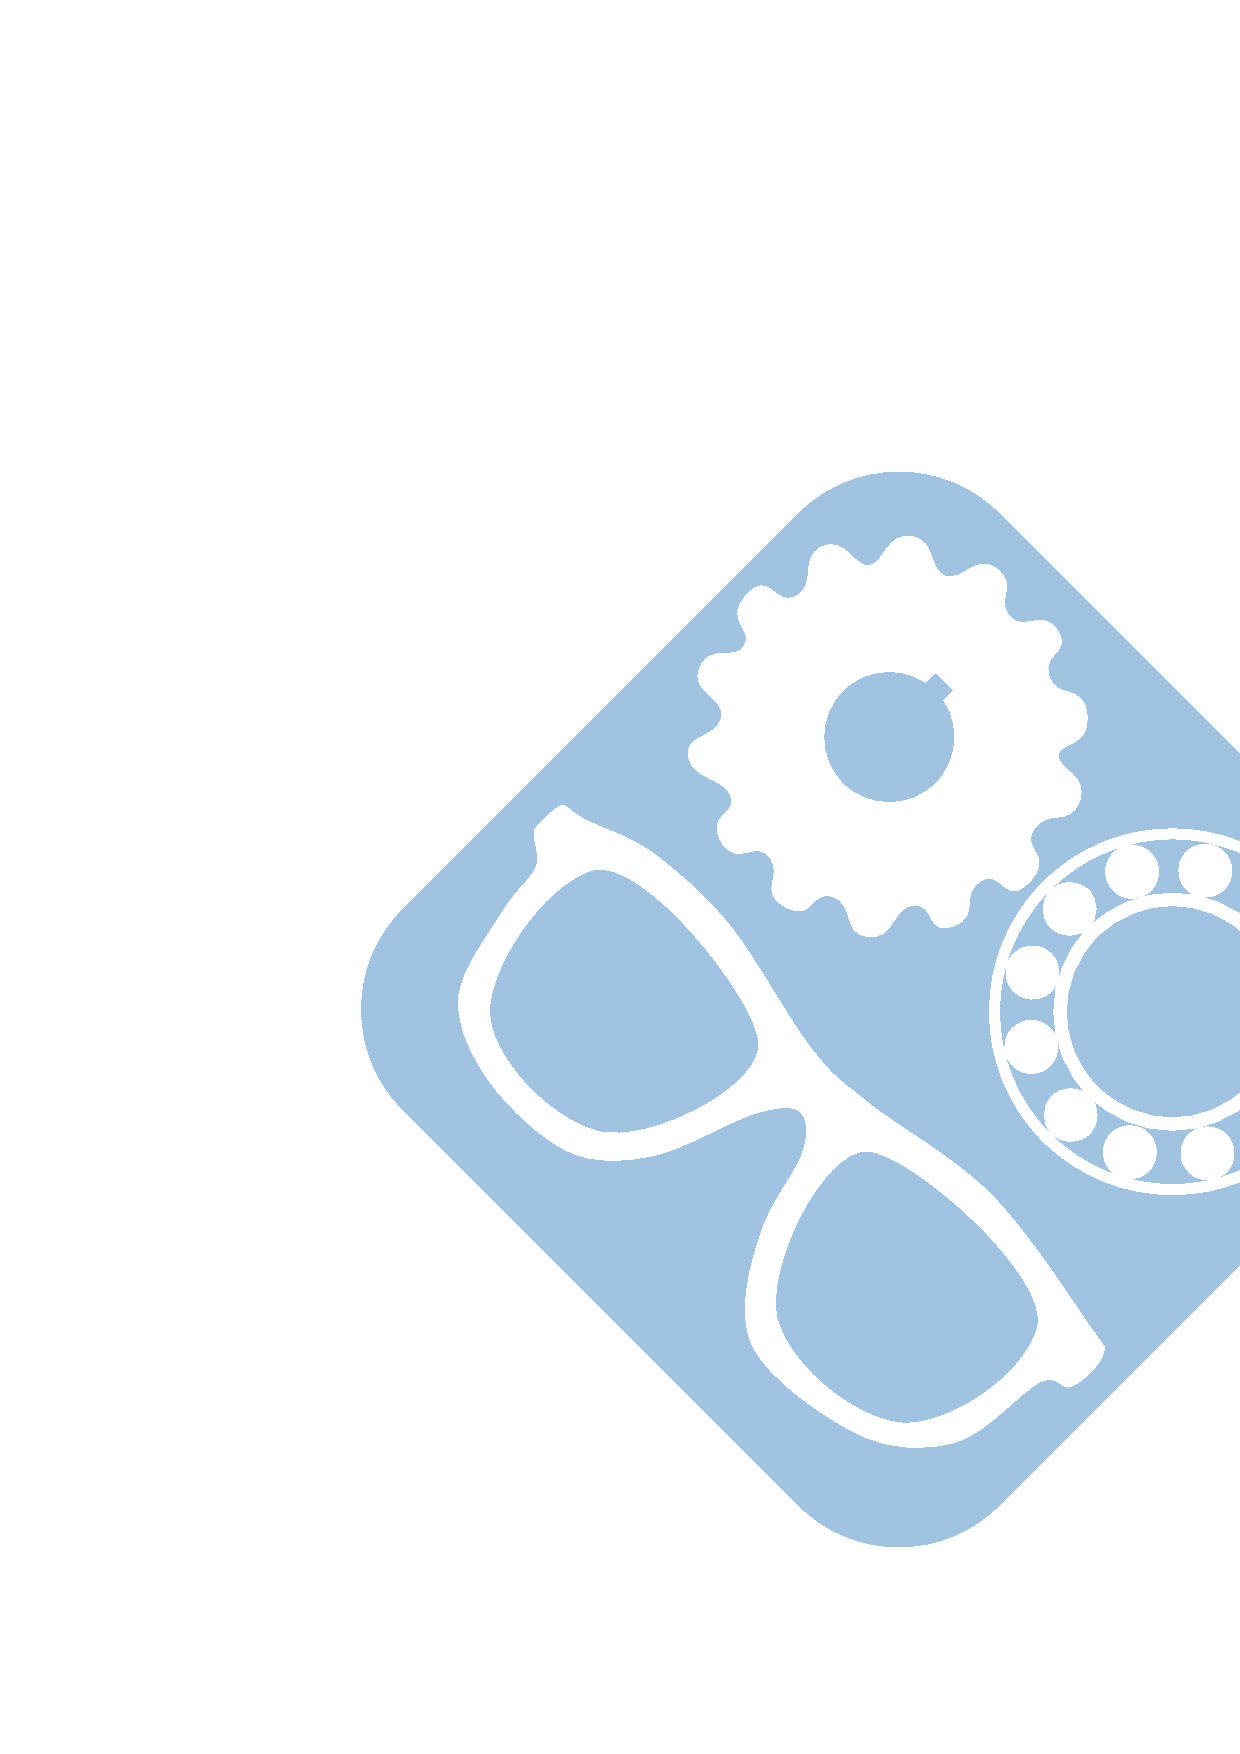
\includegraphics[width=\paperwidth,height=\paperheight,%
keepaspectratio]{../../img/fond3}%
\end{center}
\vfill
}}}

\newcommand{\BackgroundPicdeux}{%
\put(25,-30){%
\parbox[b][\paperheight]{\paperwidth}{%
\vfill
\begin{center}
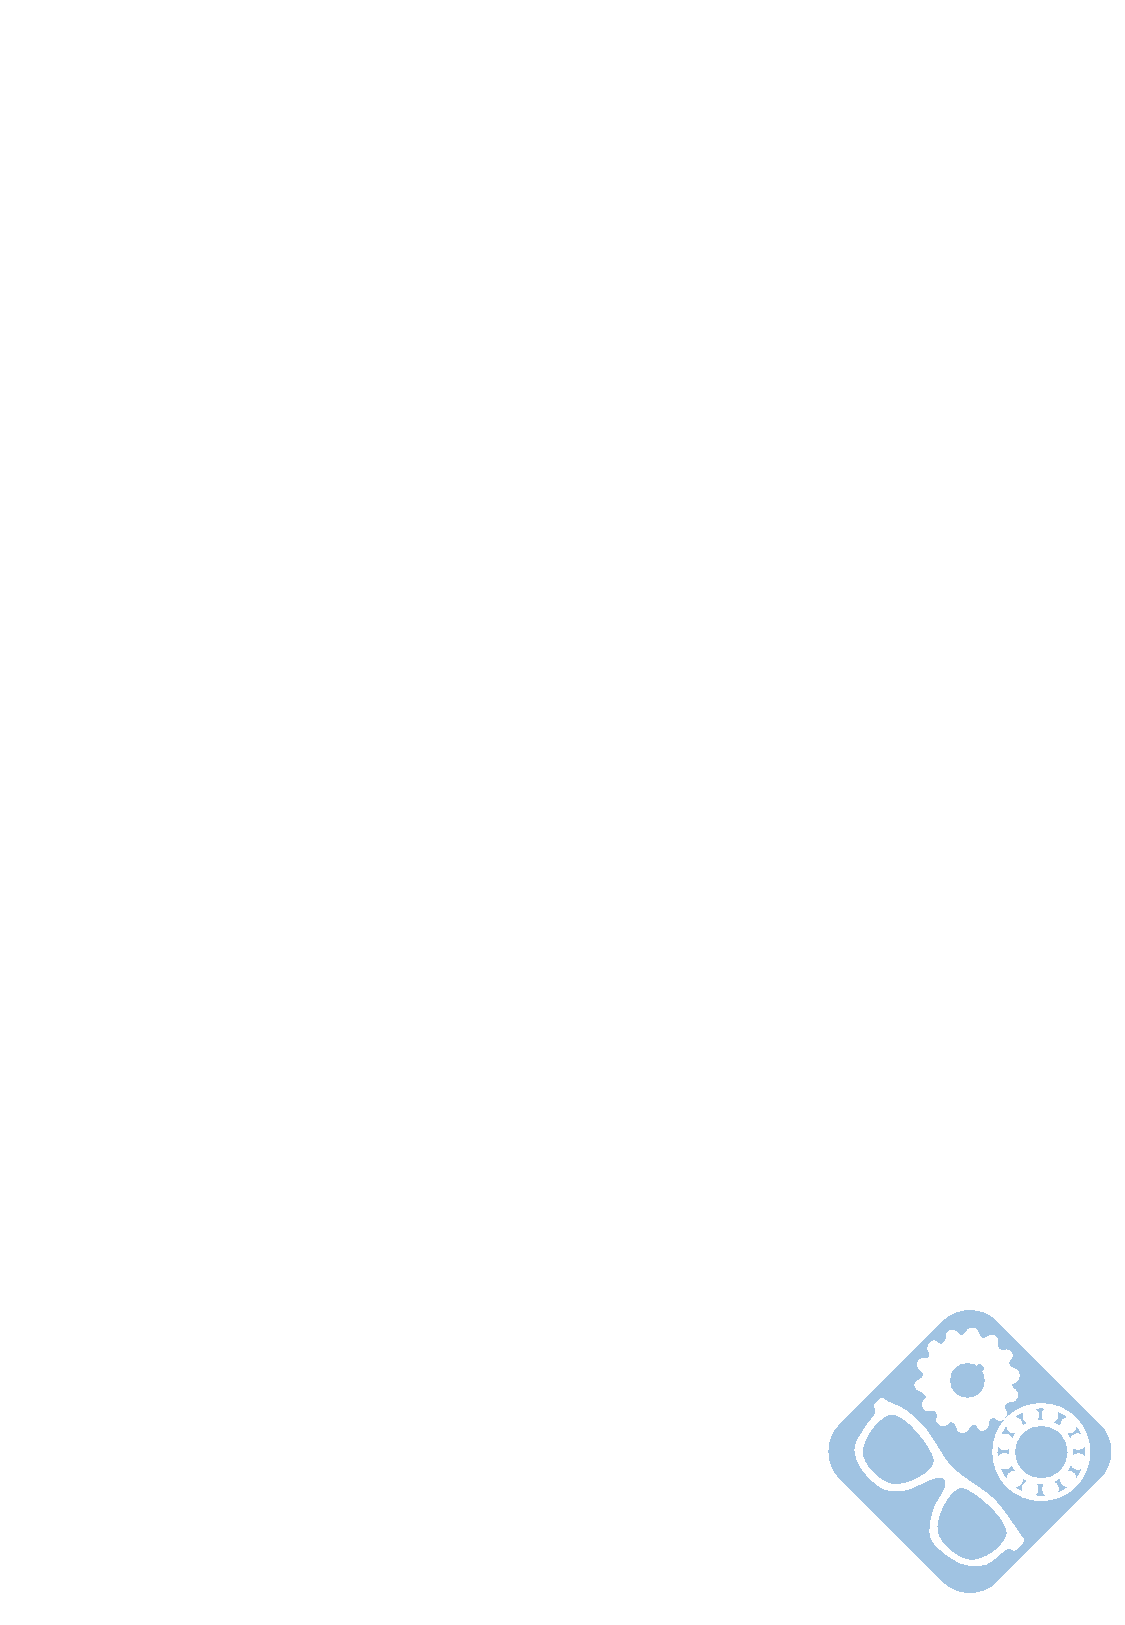
\includegraphics[width=\paperwidth,height=\paperheight,%
keepaspectratio]{../../img/fond4}%
\end{center}
\vfill
}}}

\begin{document}

\pagestyle{empty}

\vspace*{-3\baselineskip}

\AddToShipoutPicture*{\BackgroundPic}

\ifdef{\auteurdeux}{\begin{tabular}{>{\columncolor{gray!00}}m{.3\linewidth} m{.3\linewidth} >{\columncolor{gray!00}}m{.3\linewidth}}
Séquence : \sequence &  \multirow{3}{*}{\hspace{1cm}
\includegraphics[height=1.5cm]{../../img/logo}} &  \begin{flushright} \multirow{4}{*}{\hspace{1cm}
\includegraphics[height=4cm]{img/qrcode}}\end{flushright}\\
Document : \type\num \\
 \institute \\
 \auteurun\\
 \auteurdeux
\end{tabular}}{\begin{tabular}{>{\columncolor{gray!00}}m{.3\linewidth} m{.3\linewidth} >{\columncolor{gray!00}}m{.3\linewidth}}
Séquence : \sequence &  \multirow{3}{*}{\hspace{1cm}
\includegraphics[height=1.5cm]{../../img/logo}} &  \begin{flushright} \multirow{4}{*}{\hspace{1cm}
\includegraphics[height=4cm]{img/qrcode}}\end{flushright}\\
Document : \type\num \\
 \institute \\
 \auteurun
\end{tabular}}

\vspace{1cm}

\ifdef{\prive}{\begin{center}\colorbox{danger}{\Huge{Avec Correction}}\end{center}}{}

\begin{center}\huge{\nom}\end{center}

\vspace{2cm}

\ifdef{\imagedeux}{\begin{minipage}{0.49\linewidth}}{}
\begin{center}\includegraphics[height=5cm]{/home/renaud/Documents/Renaud/GitHub/django_education/systemes/\imageun}\end{center}
\ifdef{\imagedeux}{\end{minipage}\hfill
\begin{minipage}{0.49\linewidth}
\begin{center}\includegraphics[height=5cm]{/home/renaud/Documents/Renaud/GitHub/django_education/systemes/\imagedeux}\end{center}
\end{minipage}}{}

\vspace{5cm}


\begin{tabular}{p{.15\linewidth} >{\columncolor{white}}p{.8\linewidth}}
    \rowcolor{gray!20}
    Référence & S\sequence\ - \type\num \\
    Compétences & \competences \\
 	\rowcolor{gray!20}
    Description & \descrip \\
    Système & \systemes
  \end{tabular}

\newpage

\AddToShipoutPicture{\BackgroundPicdeux}

\pagestyle{normal}

\section{Boîte CATEP}

\subsection{Présentation}

\begin{figure}[!h]
\begin{minipage}{0.6\linewidth}
Une boîte de vitesses est un dispositif mécanique permettant d'adapter la transmission d'un mouvement entre un arbre moteur et un arbre récepteur. Utilisée dans de multiples contextes (machines-outils, transports routiers, etc.), son cas d'utilisation le plus fréquent est la transmission de la puissance d'un moteur thermique aux roues motrices d'un véhicule.
\end{minipage}
 \hfill
\begin{minipage}{0.35\linewidth}
 \centering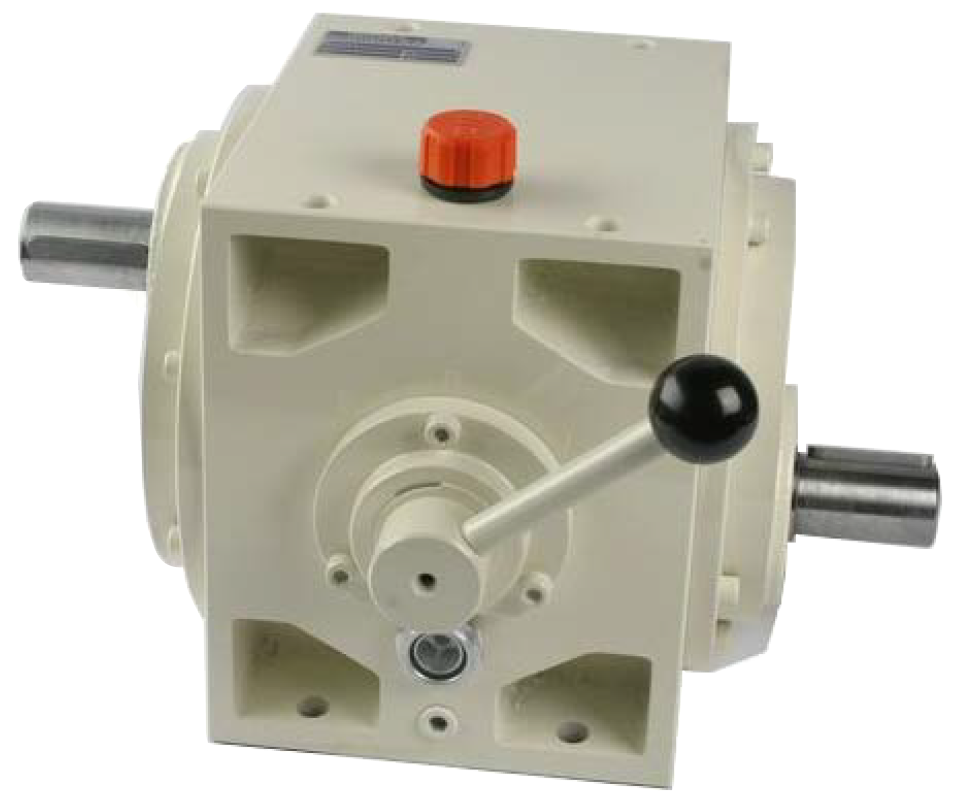
\includegraphics[width=0.9\linewidth]{img/Catep.png}
 \caption{Boîte C.A.T.E.P.}
 \label{fig1}
\end{minipage}
\end{figure}

\subsection{Les rapports de réduction}

\begin{figure}[!h]
 \centering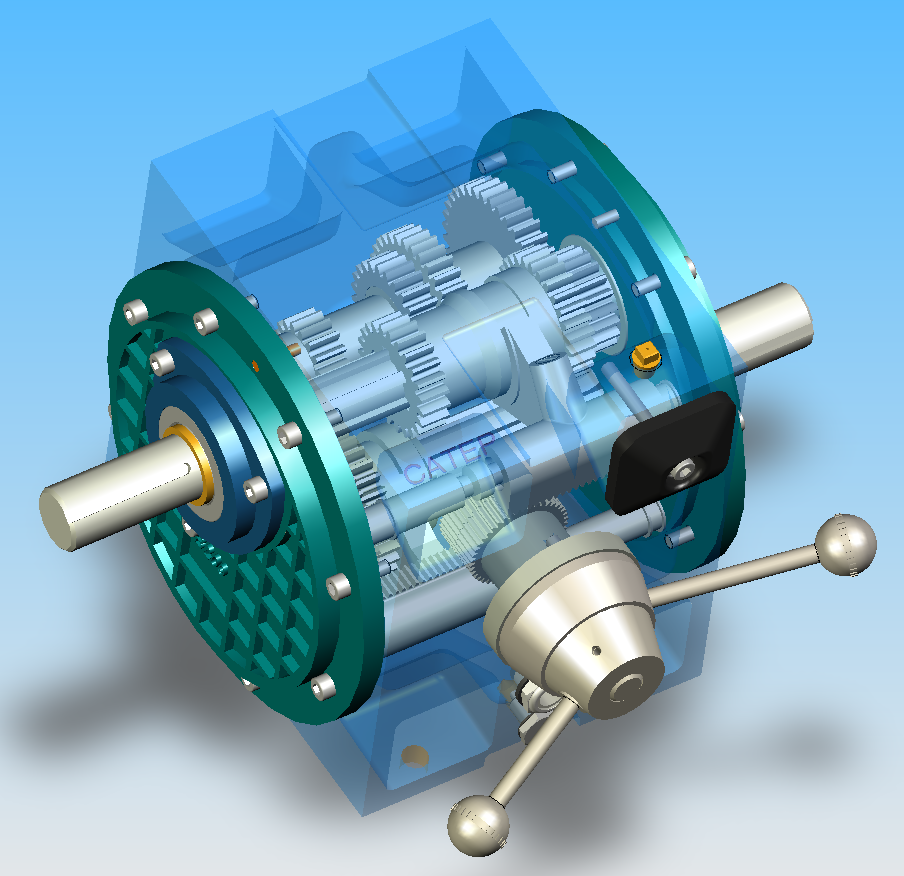
\includegraphics[width=0.6\linewidth]{img/Catep-2.png}
 \caption{Boîte ouverte}
 \label{fig2}
\end{figure}

\paragraph{Question 1:} Déterminer l'ensemble des rapports de vitesse disponibles pour cette boite de vitesse.

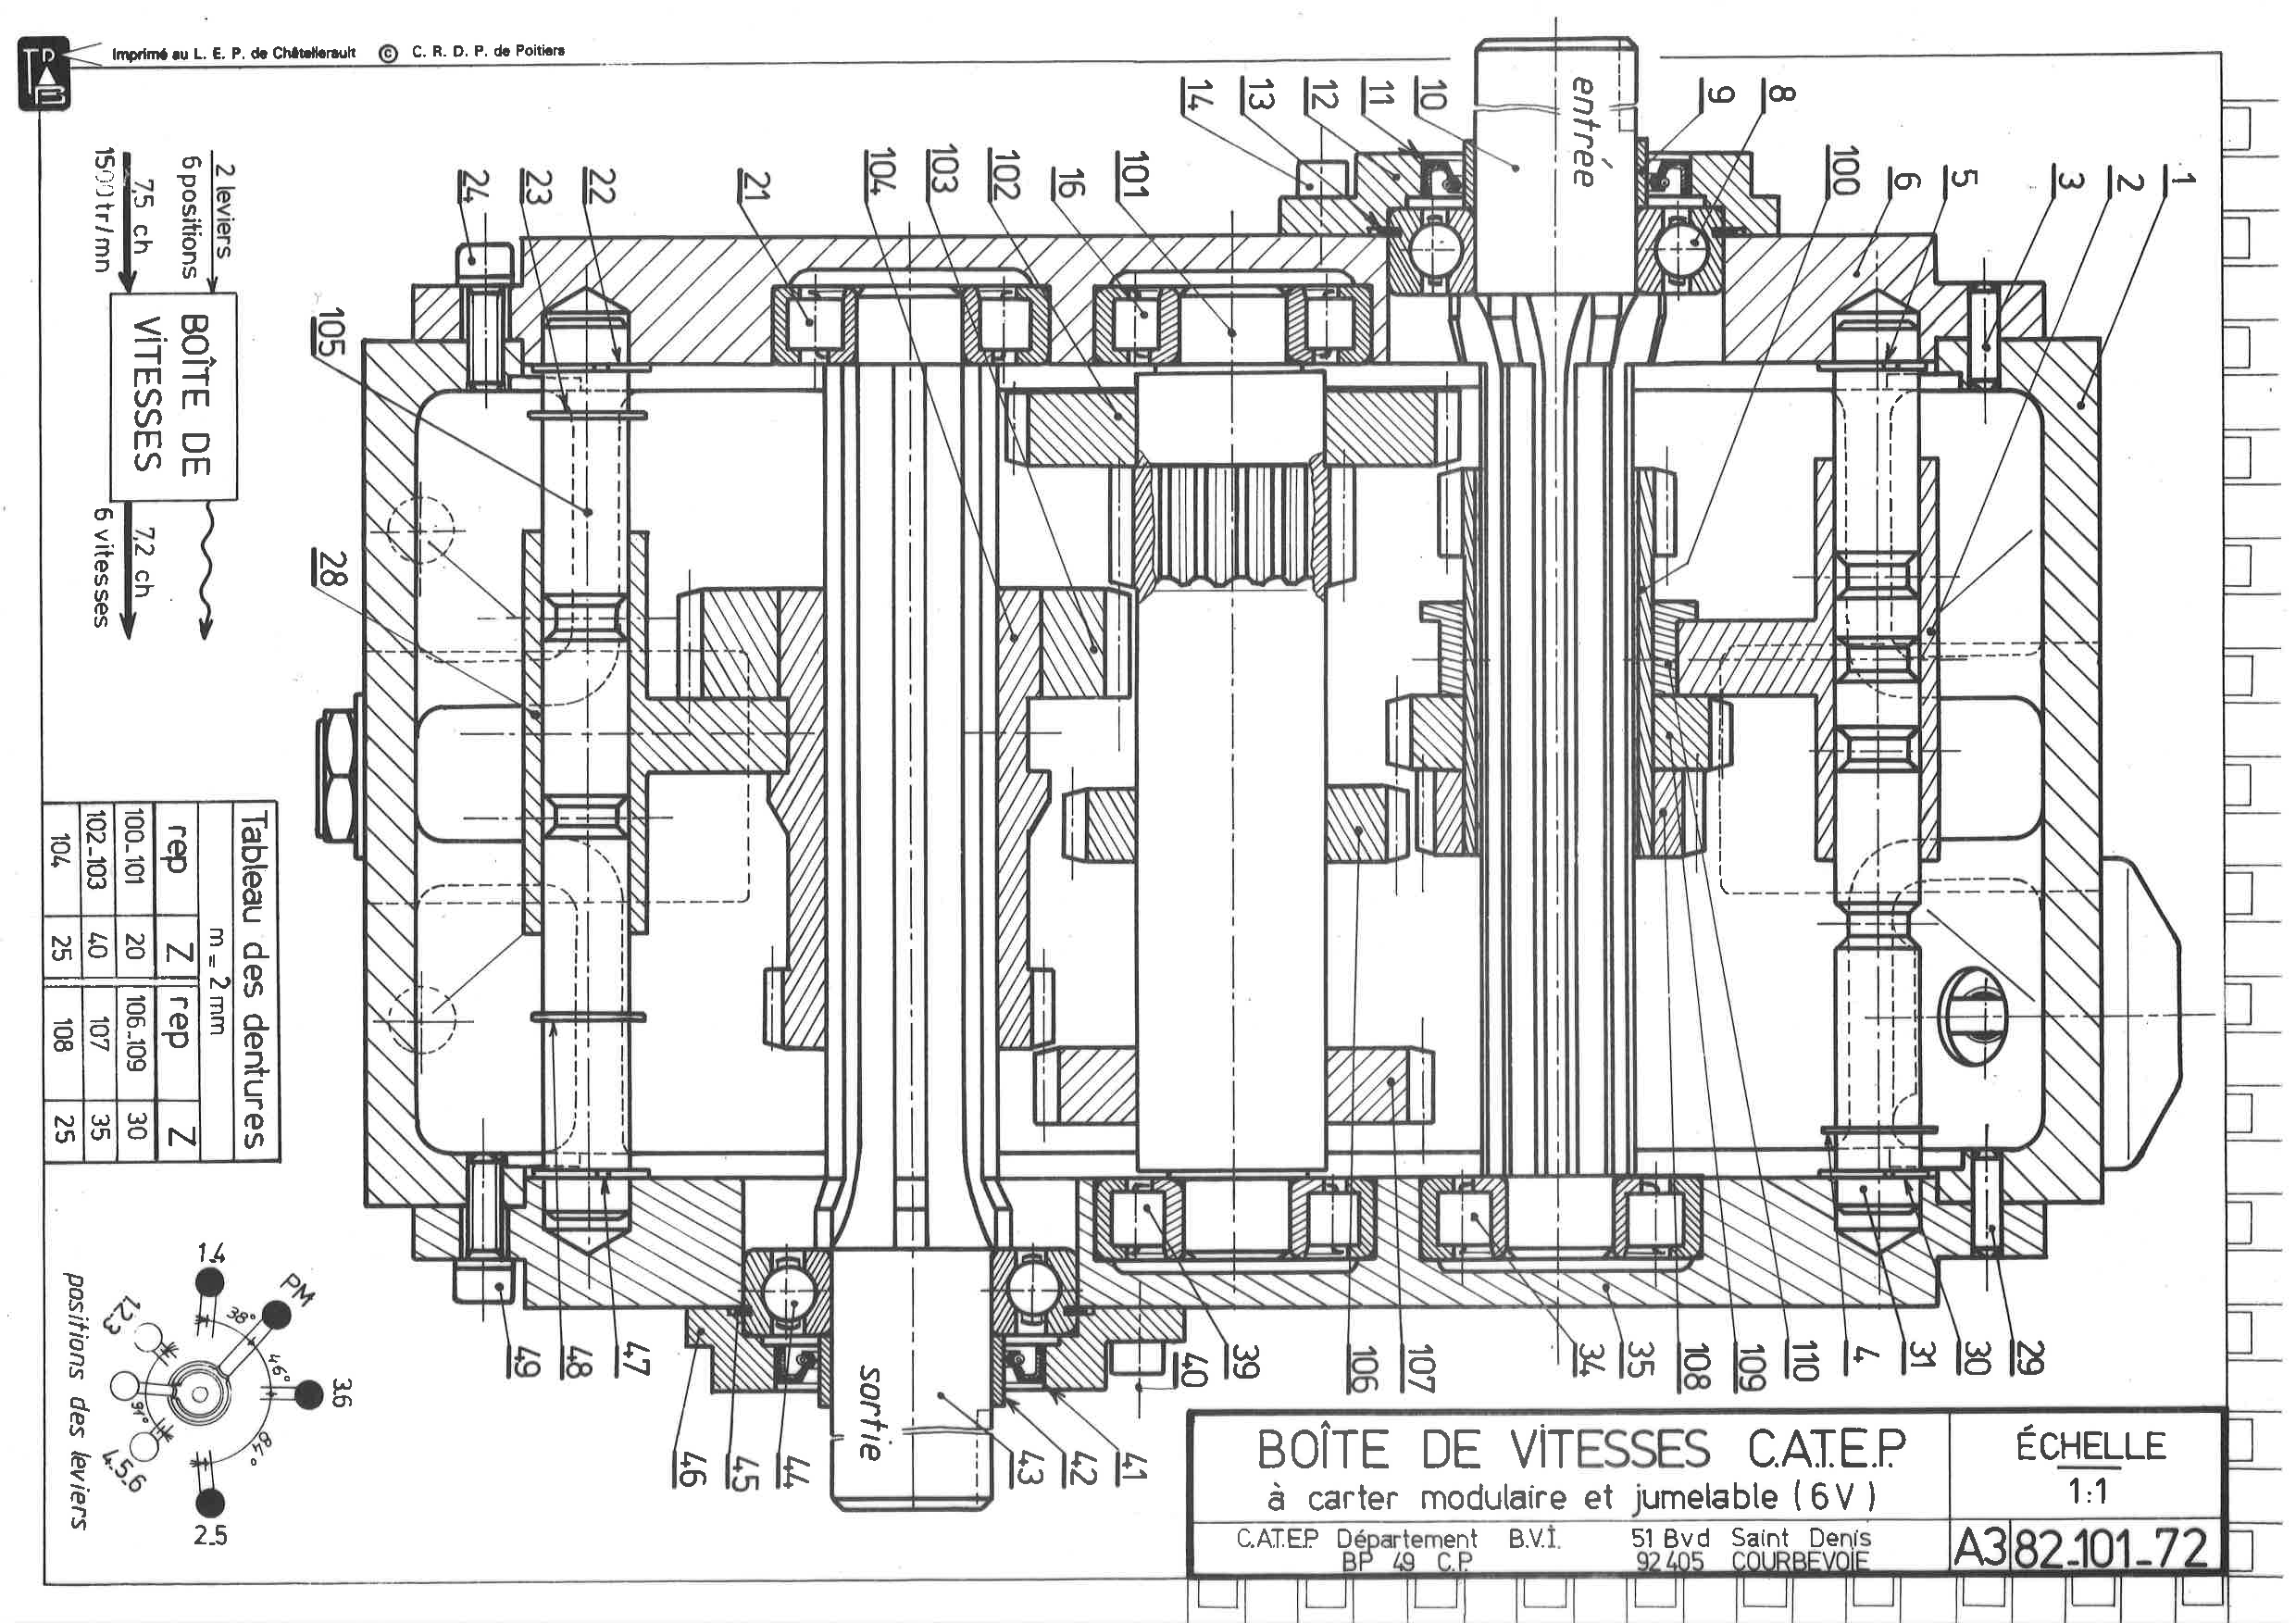
\includepdf[landscape]{img/Catep2.pdf}

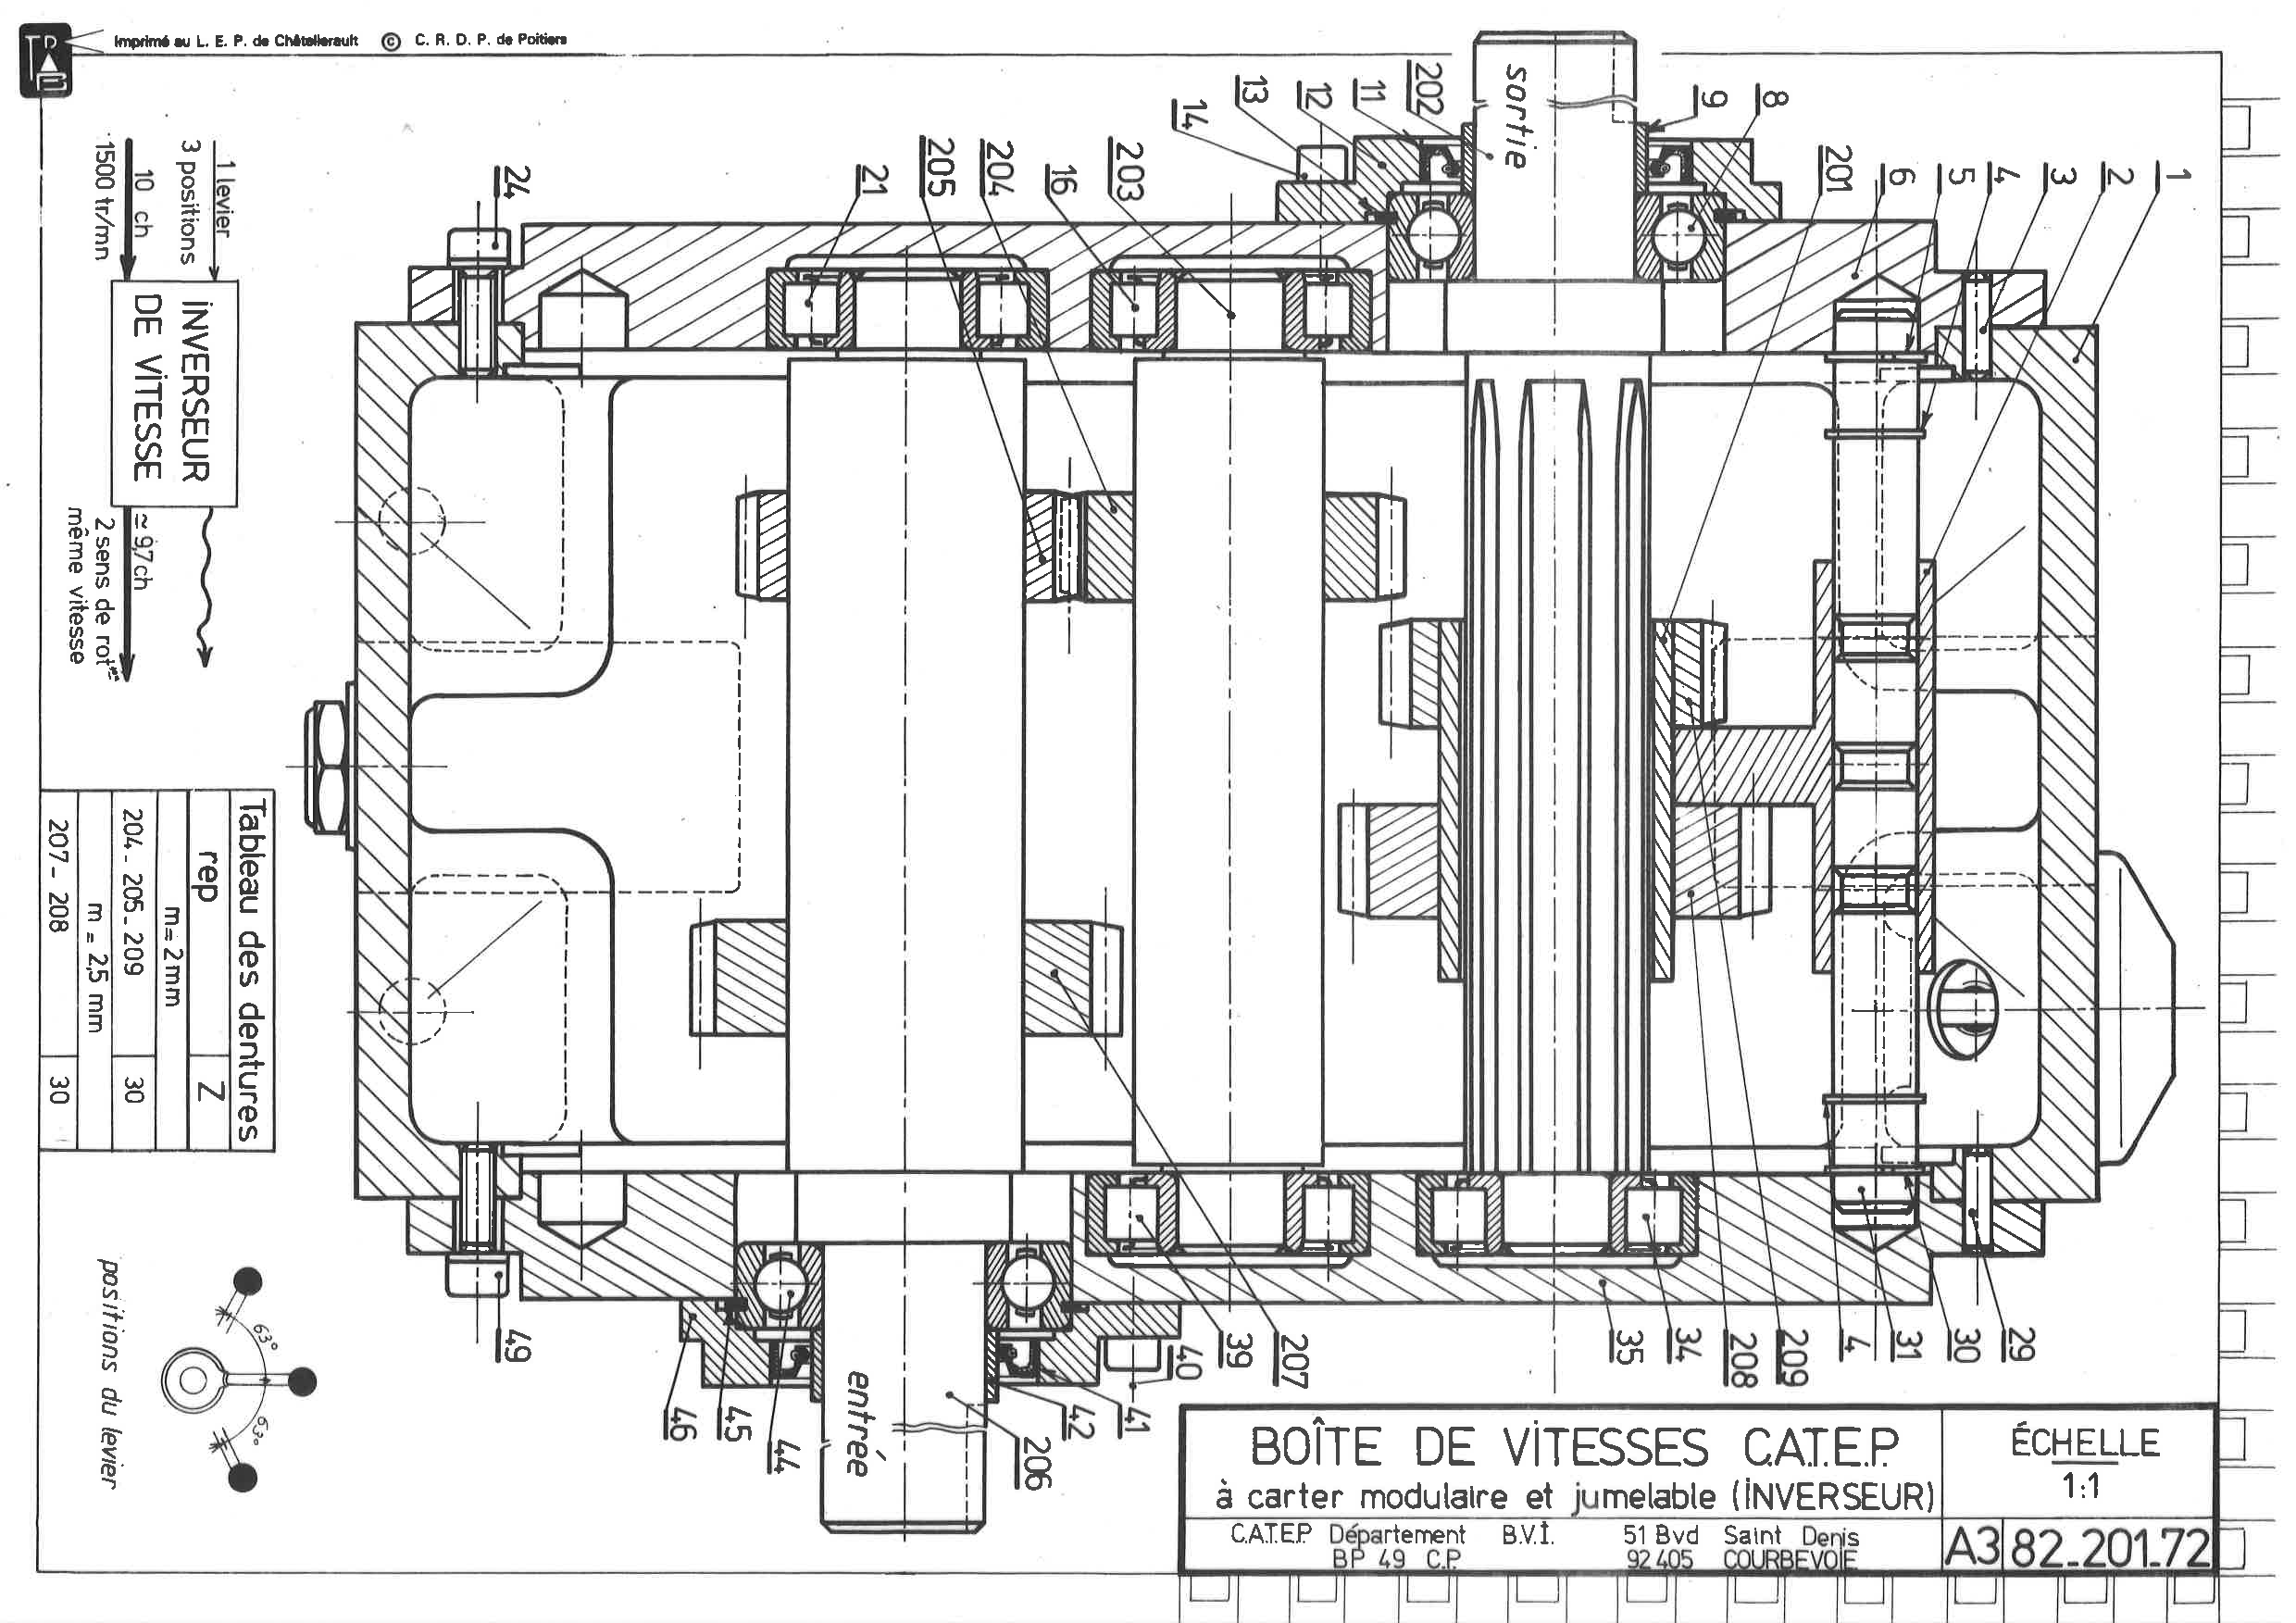
\includepdf[landscape]{img/Catep1.pdf}

\newpage

\section{Le réducteur S.N.T.}

\subsection{Présentation}

\begin{figure}[!h]
\begin{minipage}{0.6\linewidth}
Le réducteur SNT a la particularité d'être un réducteur à vis sans fin.

Avantages:
\begin{itemize}
 \item Il permet d'obtenir de grands rapports de réduction,
 \item Il permet un renvoi d'angle (axes de rotations perpendiculaires)
\end{itemize}

Inconvénients:
\begin{itemize}
 \item Il ne permet pas de choisir entre plusieurs rapports de réduction.
\end{itemize}

Données:
\begin{itemize}
 \item Vis: 1 filet,
 \item Roue: 40 dents,
 \item $\overrightarrow{\Omega_v}=\omega_v.\overrightarrow{x}$, avec $\omega_v>0$,
 \item $\overrightarrow{\Omega_r}=\omega_r.\overrightarrow{z}$.
\end{itemize}

\end{minipage}
 \hfill
\begin{minipage}{0.35\linewidth}
 \centering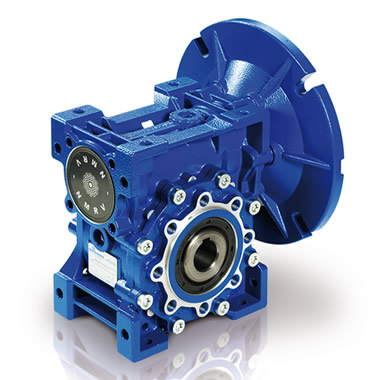
\includegraphics[width=0.9\linewidth]{img/SNT.jpg}
 \caption{Réducteur SNT}
 \label{fig3}
\end{minipage}
\end{figure}

\subsection{la réduction}

\paragraph{Question 1:} Déterminer le signe de $\omega_r$ et le rapport de réduction de ce réducteur S.N.T.

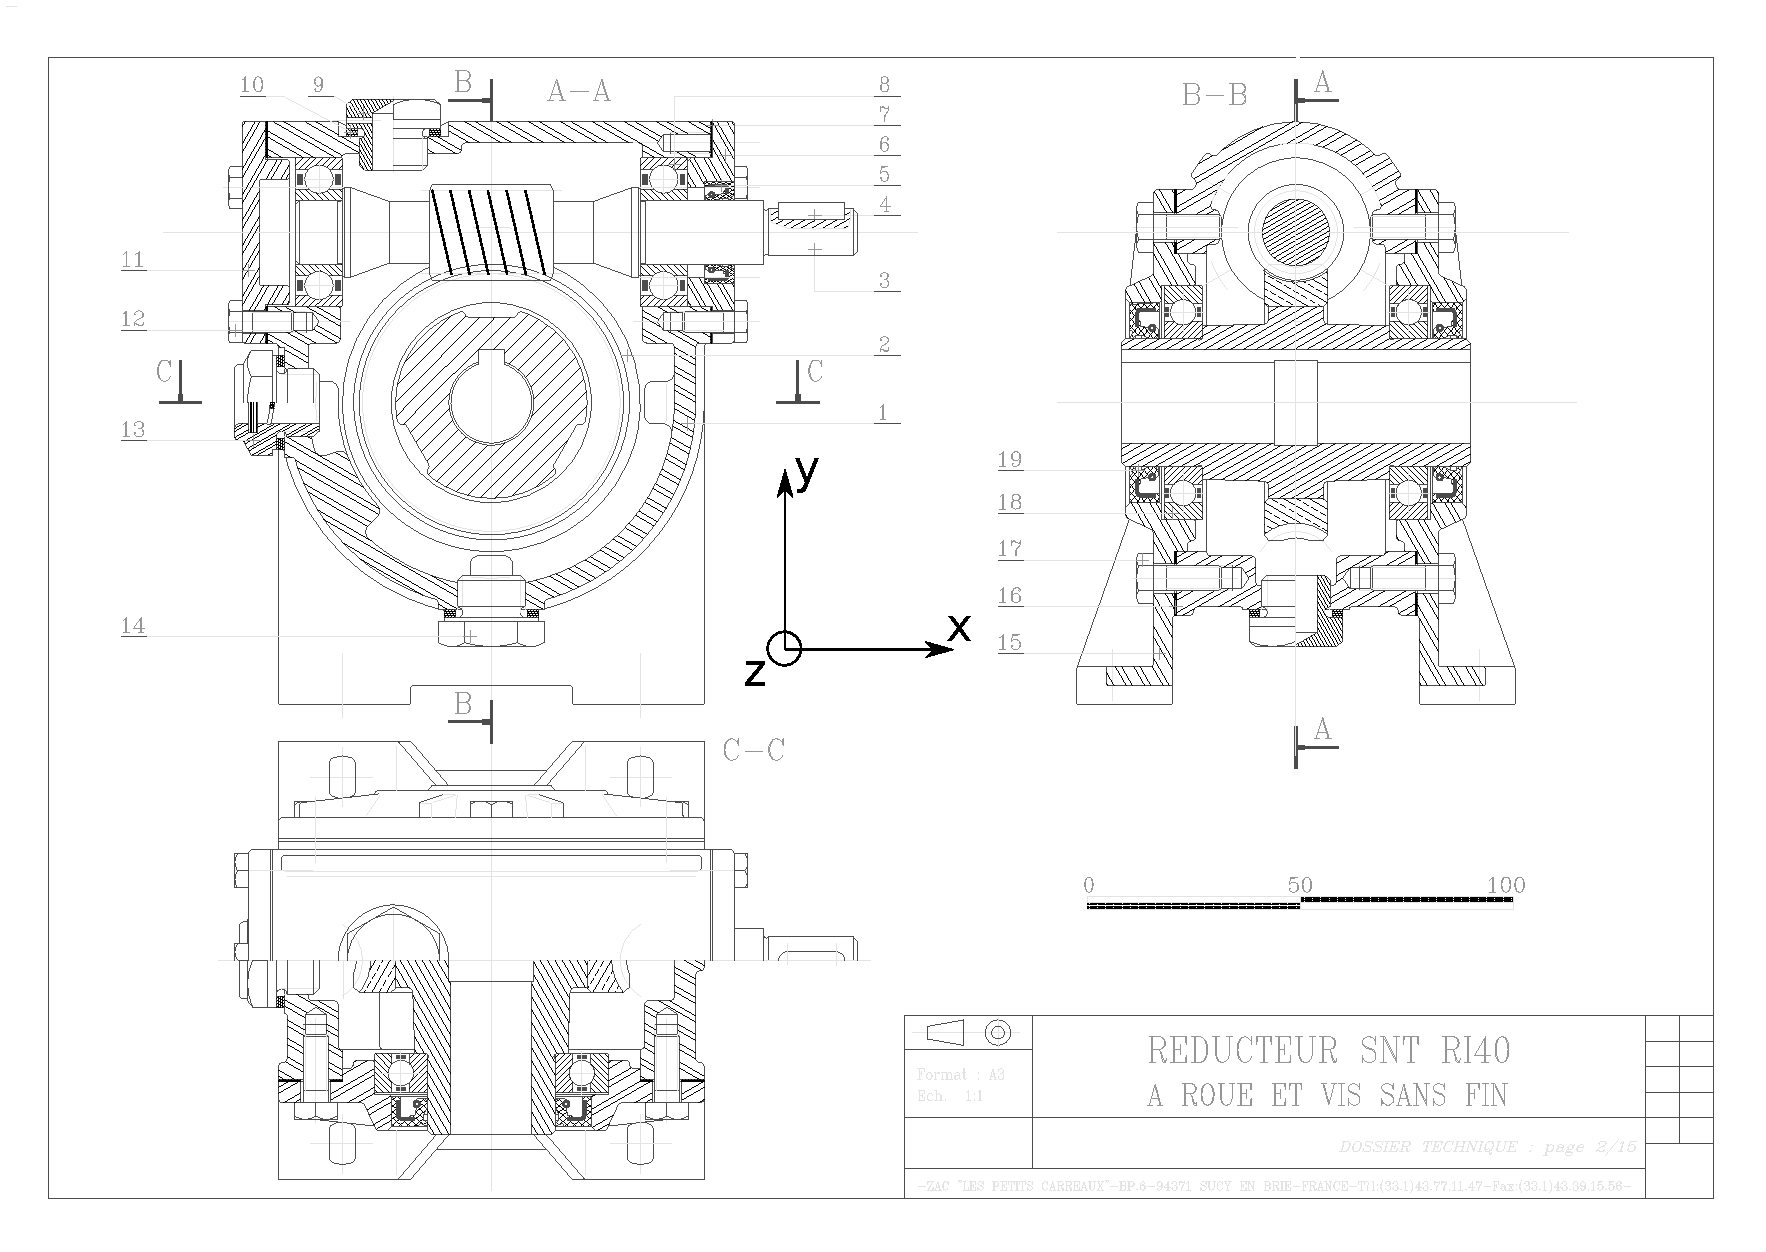
\includepdf[landscape]{img/Reducteur_SNT.pdf}

\newpage

\section{Palan Eurochain VL5}


\subsection{Présentation}

\begin{figure}[!h]
\begin{minipage}{0.6\linewidth}

L'EUROCHAIN VL est un palan électrique de la société VERLINDE répondant à des besoins de levage industriel de petite et moyenne capacité (160 à 5000 kg).

L'EUROCHAIN VL se combine avec des chariots à déplacement manuel ou électrique installés sur monorail, potence ou pont roulant.
\end{minipage}
 \hfill
\begin{minipage}{0.35\linewidth}
 \centering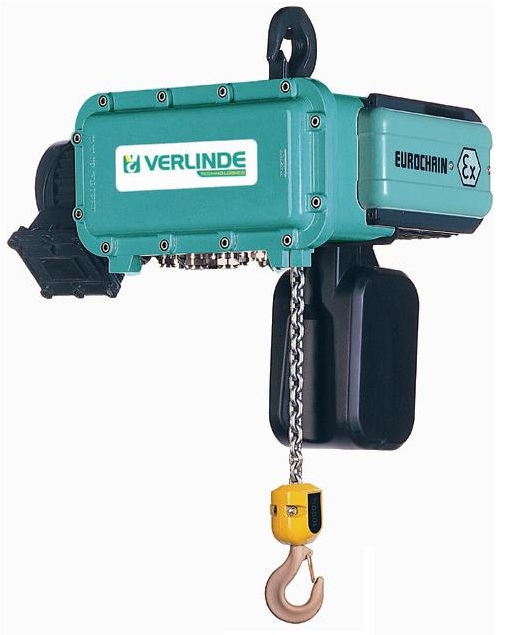
\includegraphics[width=0.7\linewidth]{img/eurochain.jpg}
 \caption{Palan Eurochain}
 \label{fig4}
\end{minipage}
\end{figure}

Caractéristiques générales :
\begin{itemize}
 \item Réducteur à double train épicycloïdal (Rapport de transmission global : $i_{global}=1/43$),
 \item Capacité de charge de $160$ à $5000kg$,
 \item Couple nominal du moteur électrique : $Cn=5,6Nm$,
 \item Vitesse de levage de la charge : $v=4m.mn^{-1}$ ou $0,066m.s^{-1}$,
 \item Hauteur de levage de $3$ à $30m$,
 \item Levage mono-vitesse ou bi-vitesse,
 \item Déplacement horizontal manuel ou électrique (mono-vitesse, bi-vitesse ou vitesse variable),
 \item Diamètre primitif d'enroulement de la chaîne sur la noix de levage 5 :  $\Phi_{noix}=41mm$,
 \item Rendement du mécanisme de transmission de puissance : $\eta=0,84$.
\end{itemize}

~\

Caractéristiques de sécurité :
\begin{itemize}
 \item Commande très basse tension (48 V ),
 \item Marche-arrêt de type coup de poing,
 \item Limiteur de couple (disque de limiteur 28 : $R_{ext}=34mm$, $R_{int}=22mm$, facteur de frottement : $\mu=0,4$),
 \item Frein de levage à disque,
 \item Matériau du ressort de freinage 32 : 50 Cr V 4,
 \item Disque de freinage 30 ($R_{ext}=42,5 mm$, $R_{int}=30mm$, facteur de frottement : $\mu=0,4$),
 \item Conforme à la directive CE relative aux machines 89/392/CEE,
 \item Couple maxi sur l'arbre 2 : $C_{max}=7,3Nm$,
 \item Caractéristiques de l'arbre canneluré 2 (Matériau : 35 Cr Mo 4, Coefficient de sécurité adopté par le constructeur : s = 5).
\end{itemize} 

\newpage


\begin{figure}[!h]
 \centering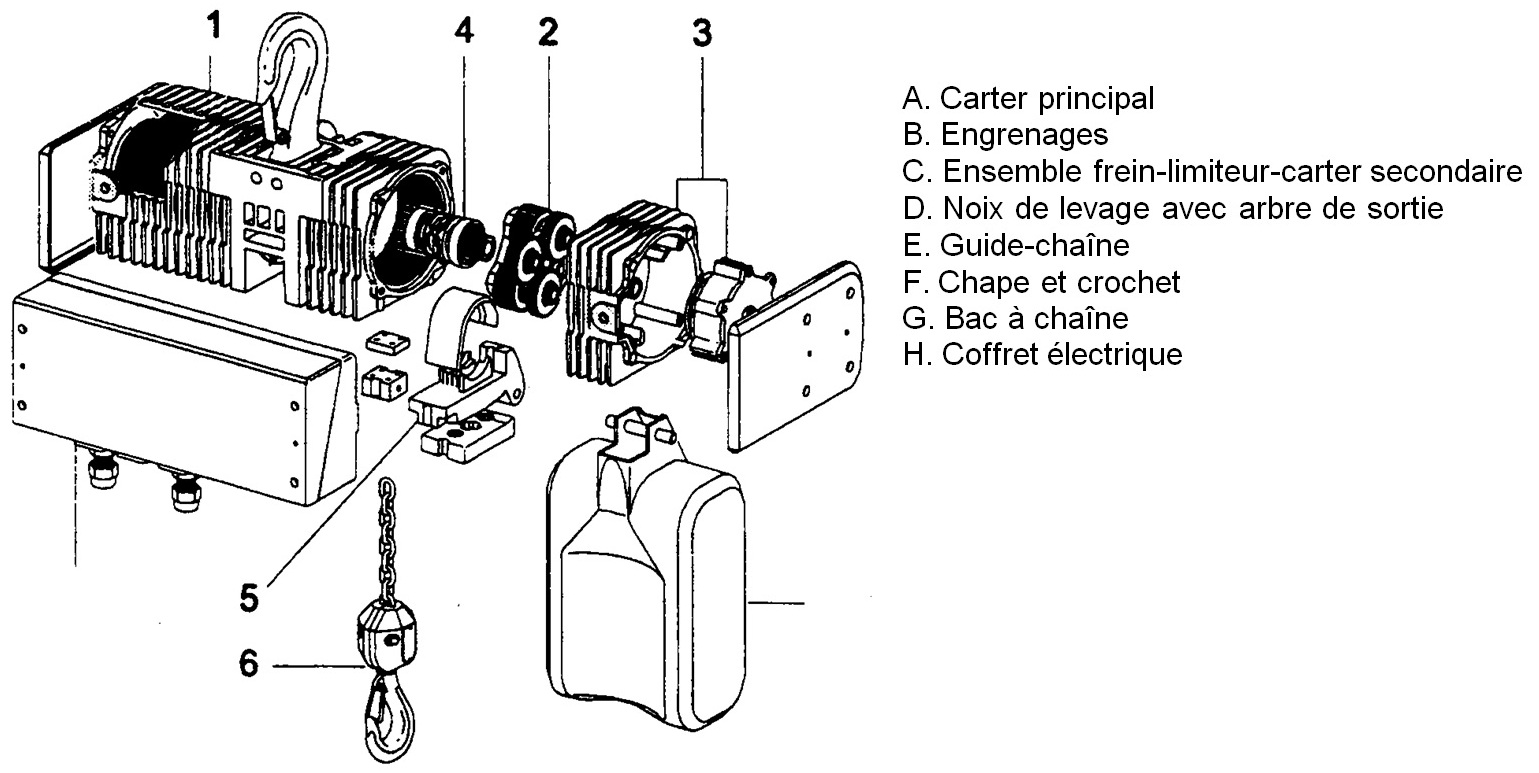
\includegraphics[width=0.6\linewidth]{img/eurochain_1.jpg}
 \centering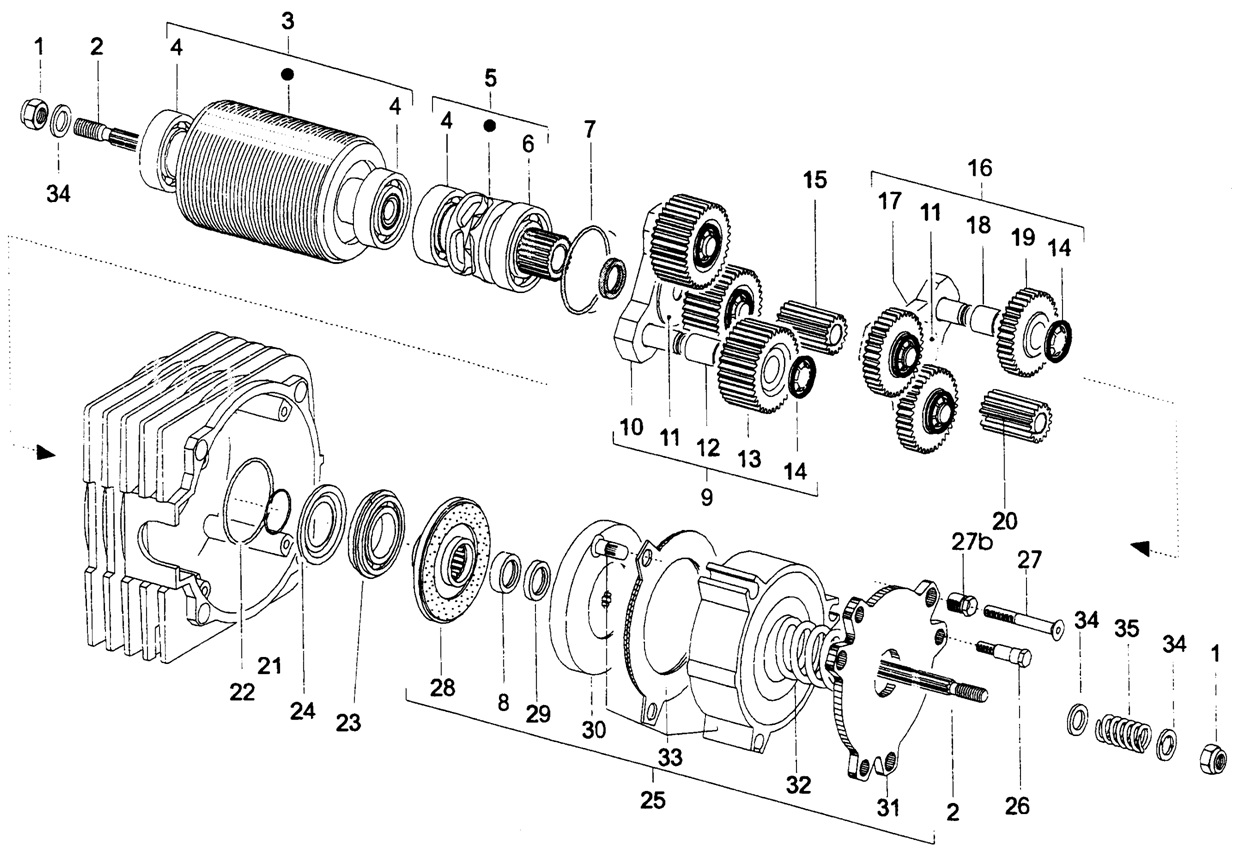
\includegraphics[width=0.6\linewidth]{img/eurochain_2.jpg}
 \caption{Sous-ensembles du Palan}
 \label{fig5}
\end{figure}

 \begin{tabular}{|c|c|c|c|c|c|}
 \hline
 R & N & Désignation & R & N & Désignation \\
 \hline
 1 & 2 & Ecrou autofreiné M8 & 21 & 1 & Anneau élastique \\
 \hline
 2 & 1 & Arbre de transmission & 22 & 1 & Joint torique $\Phi2\times47$ NB70 \\
 \hline
 3 & 1 & Rotor assemblé & 23 & 1 & Roulement 6005 2NSLNR \\
 \hline
 4 & 3 & Roulement 6004 2RS1 & 24 & 1 & Joint métallique 6005 AV \\
 \hline
 5 & 1 & Noix de levage assemblée & 25 & 1 & Frein limiteur assemblé \\
 \hline
 6 & 1 & Roulement 6005 2RS1 & 26 & 3 & Vis de fixation \\
 \hline
 7 & 1 & Bague de limiteur & 27 & 3 & Vis de blocage \\
 \hline
 8 & 1 & Bague d'étanchéité & 27b & 1 & Ecrou de réglage \\
 \hline
 9 & 1 & Ensemble satellite 2ème étage & 28 & 1 & Disque limiteur assemblé \\
 \hline
 10 & 1 & Porte-satellite & 29 & 1 & Joint à lévre \\
 \hline
 11 & 2 & Rondelle laiton & 30 & 1 & Disque de frein assemblé \\
 \hline
 12 & 3 & Bague auto-lubrifiante & 31 & 1 & Disque d'ancrage \\
 \hline
 13 & 3 & Satellite 2ème étage & 32 & 1 & Ressort de frein \\
 \hline
 14 & 6 & Rondelle de retenue & 33 & 1 & Electo-aimant assemblé \\
 \hline
 15 & 1 & Planétaire 2ème étage & 34 & 3 & Rondelle \\
 \hline
 16 & 1 & Ensemble satellite 1er étage & 35 & 1 & Ressort de limiteur \\
 \hline
 17 & 1 & Porte-satellite 1er étage & 36 & 1 & Carter assemblé (Z=86, m=1,25) \\
 \hline
 18 & 3 & Bague auto-lubrifiante &  &  &  \\
 \hline
 19 & 3 & Satellite 1er étage (Z=35, m=1,25) &  &  &  \\
 \hline
 20 & 1 & Planétaire 1er  étage(Z=16, m=1,25) &  &  &  \\
 \hline
\end{tabular}

\newpage

\begin{figure}[!h]
 \centering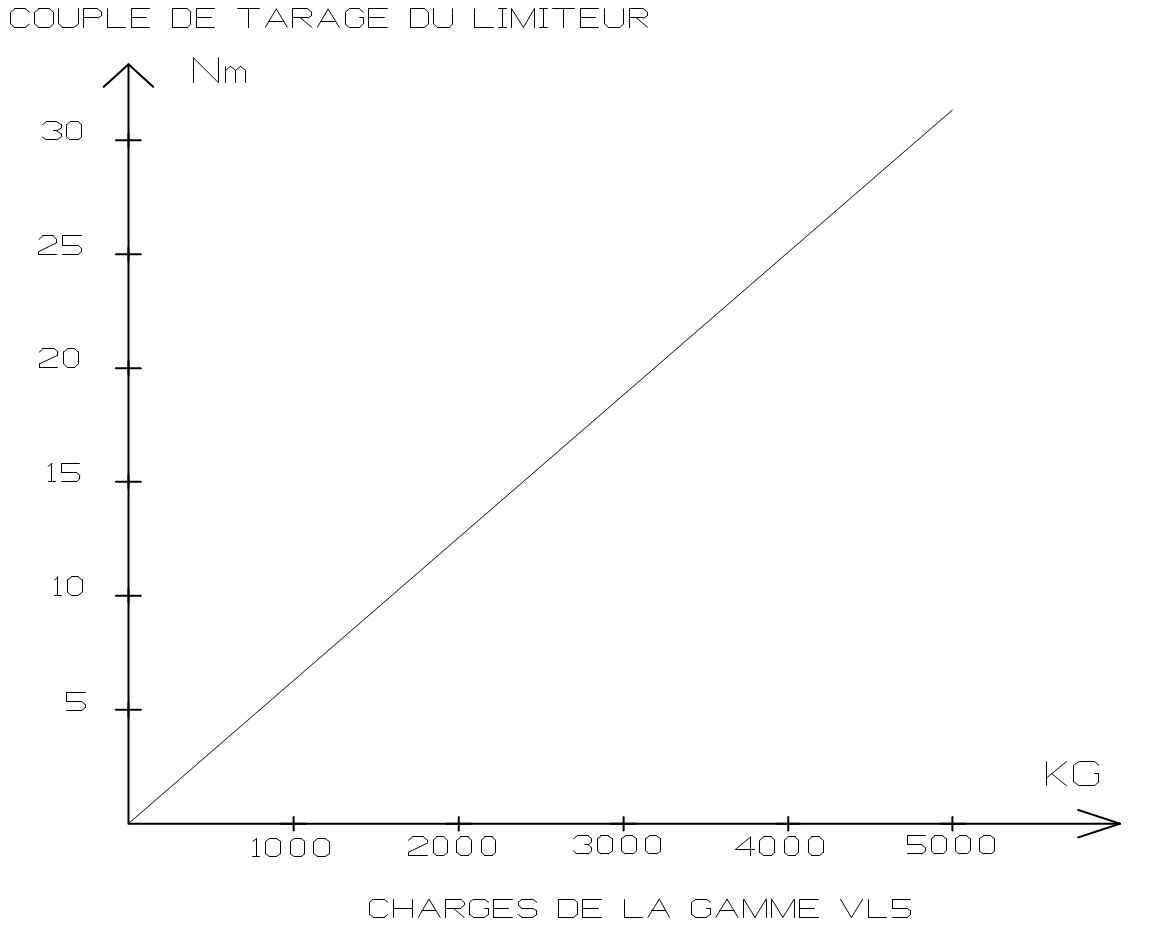
\includegraphics[width=0.8\linewidth]{img/eurochain_3.jpg}
 \centering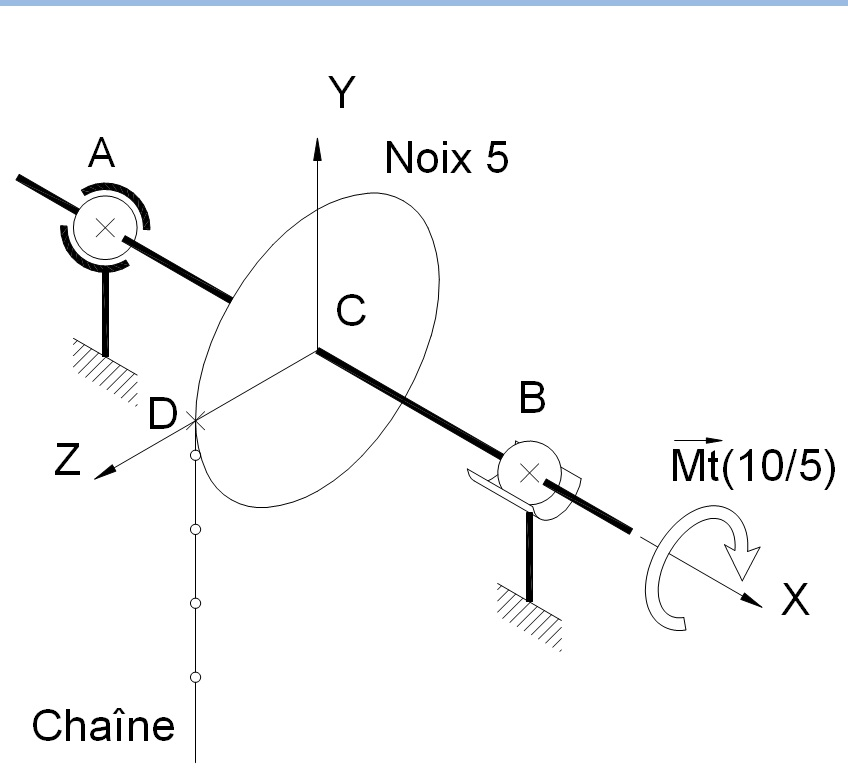
\includegraphics[width=0.8\linewidth]{img/eurochain_4.jpg}
\end{figure}

\newpage

\begin{figure}[!h]
\begin{minipage}{0.48\linewidth}
\begin{itemize}
 \item L'ensemble disque-frein (30) est en liaison glissière par rapport à l'arbre de transmission (2), grâce à des cannelures,
 \item Le reste du frein est lié en rotation  par rapport au carter.
 \item FREIN :
 \begin{enumerate}
  \item Le ressort (35) maintient en pression (30) sur (28). L'écrou (1) maintient l'ensemble sur (2),
 \item Pendant la montée ou la descente, la bobine (33) est sous tension et elle est plaquée sur le disque d'ancrage (31),
 \item Un jeu X' est prévu à cet effet,
 \item Les disques (28) et (30) tournent librement et peuvent entraîner en rotation le planétaire (20),
 \item Il y a freinage lorsque la bobine n'est plus alimentée et que le ressort (32) repousse (33) et sa garniture sur le disque de frein (30) (voir figure \ref{fig6}),
 \end{enumerate}
 \item LIMITEUR :
 \begin{enumerate}
 \item Si la charge à soulever est excessive, il se produit un glissement entre (30) et (28). Cela permet de préserver l'ensemble du système contre toute rupture intempestive,
 \item Le seuil de déclenchement du limiteur (couple de tarage) se règle grâce à l'écrou (1). Ce seuil est égal à 1,25 fois la charge nominale du palan 
(voir figure \ref{fig7}).
 \end{enumerate}
 \end{itemize}
\end{minipage}
 \hfill
\begin{minipage}{0.5\linewidth}
\centering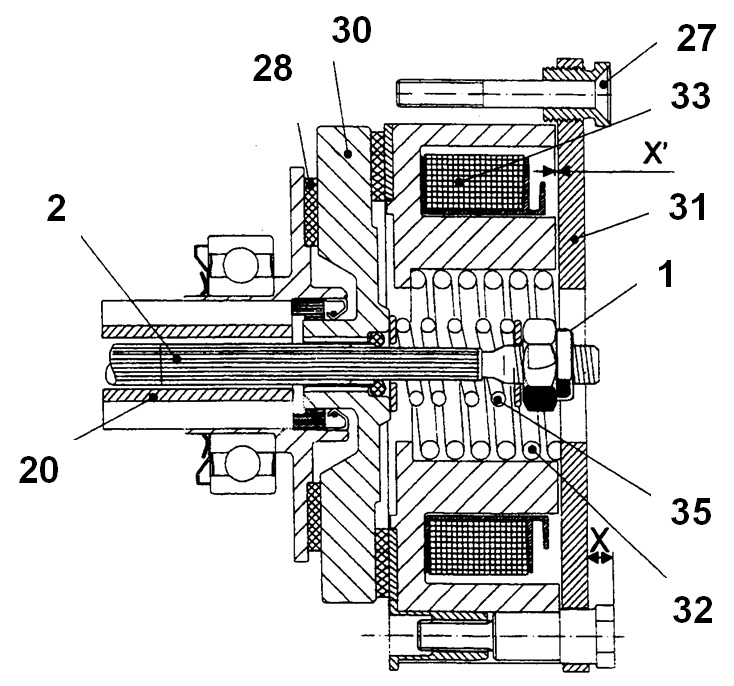
\includegraphics[width=\linewidth]{img/eurochain_5.jpg}
  \caption{Frein}
 \label{fig6}

 ~\
 
 \centering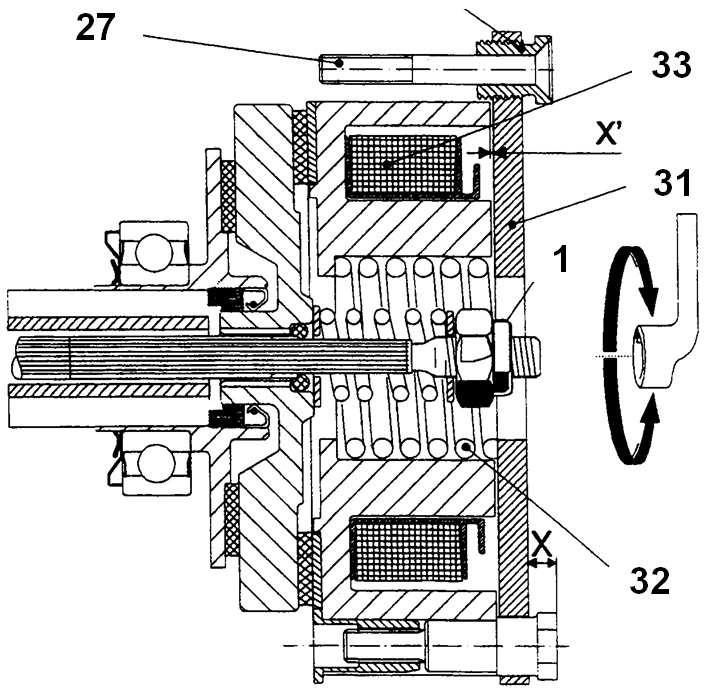
\includegraphics[width=\linewidth]{img/eurochain_6.jpg}
 \caption{Limiteur}
 \label{fig7}
\end{minipage}
\end{figure}

\newpage

\begin{figure}[!ht]
 \centering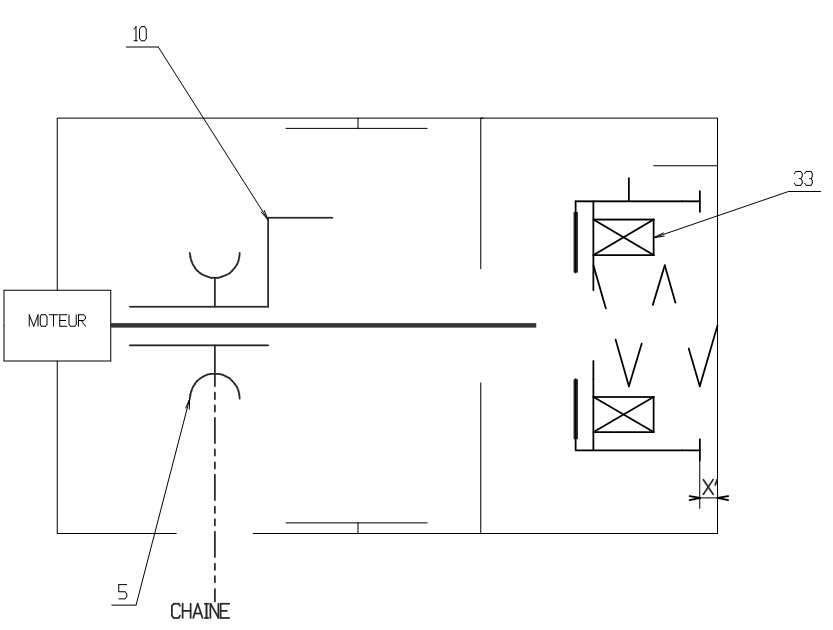
\includegraphics[width=1\linewidth]{img/eurochain_7.jpg}
 \label{fig75}
\end{figure}

\paragraph{Question 1:} Expliquer le ou les fonctionnements de ce système.

\paragraph{Question 2:} Réaliser sur la figure \ref{fig75} le schéma technologique de ce système.

\paragraph{Question 3:} Déterminer le rapport de réduction de la chaîne d'engrenage de ce système.

\newpage

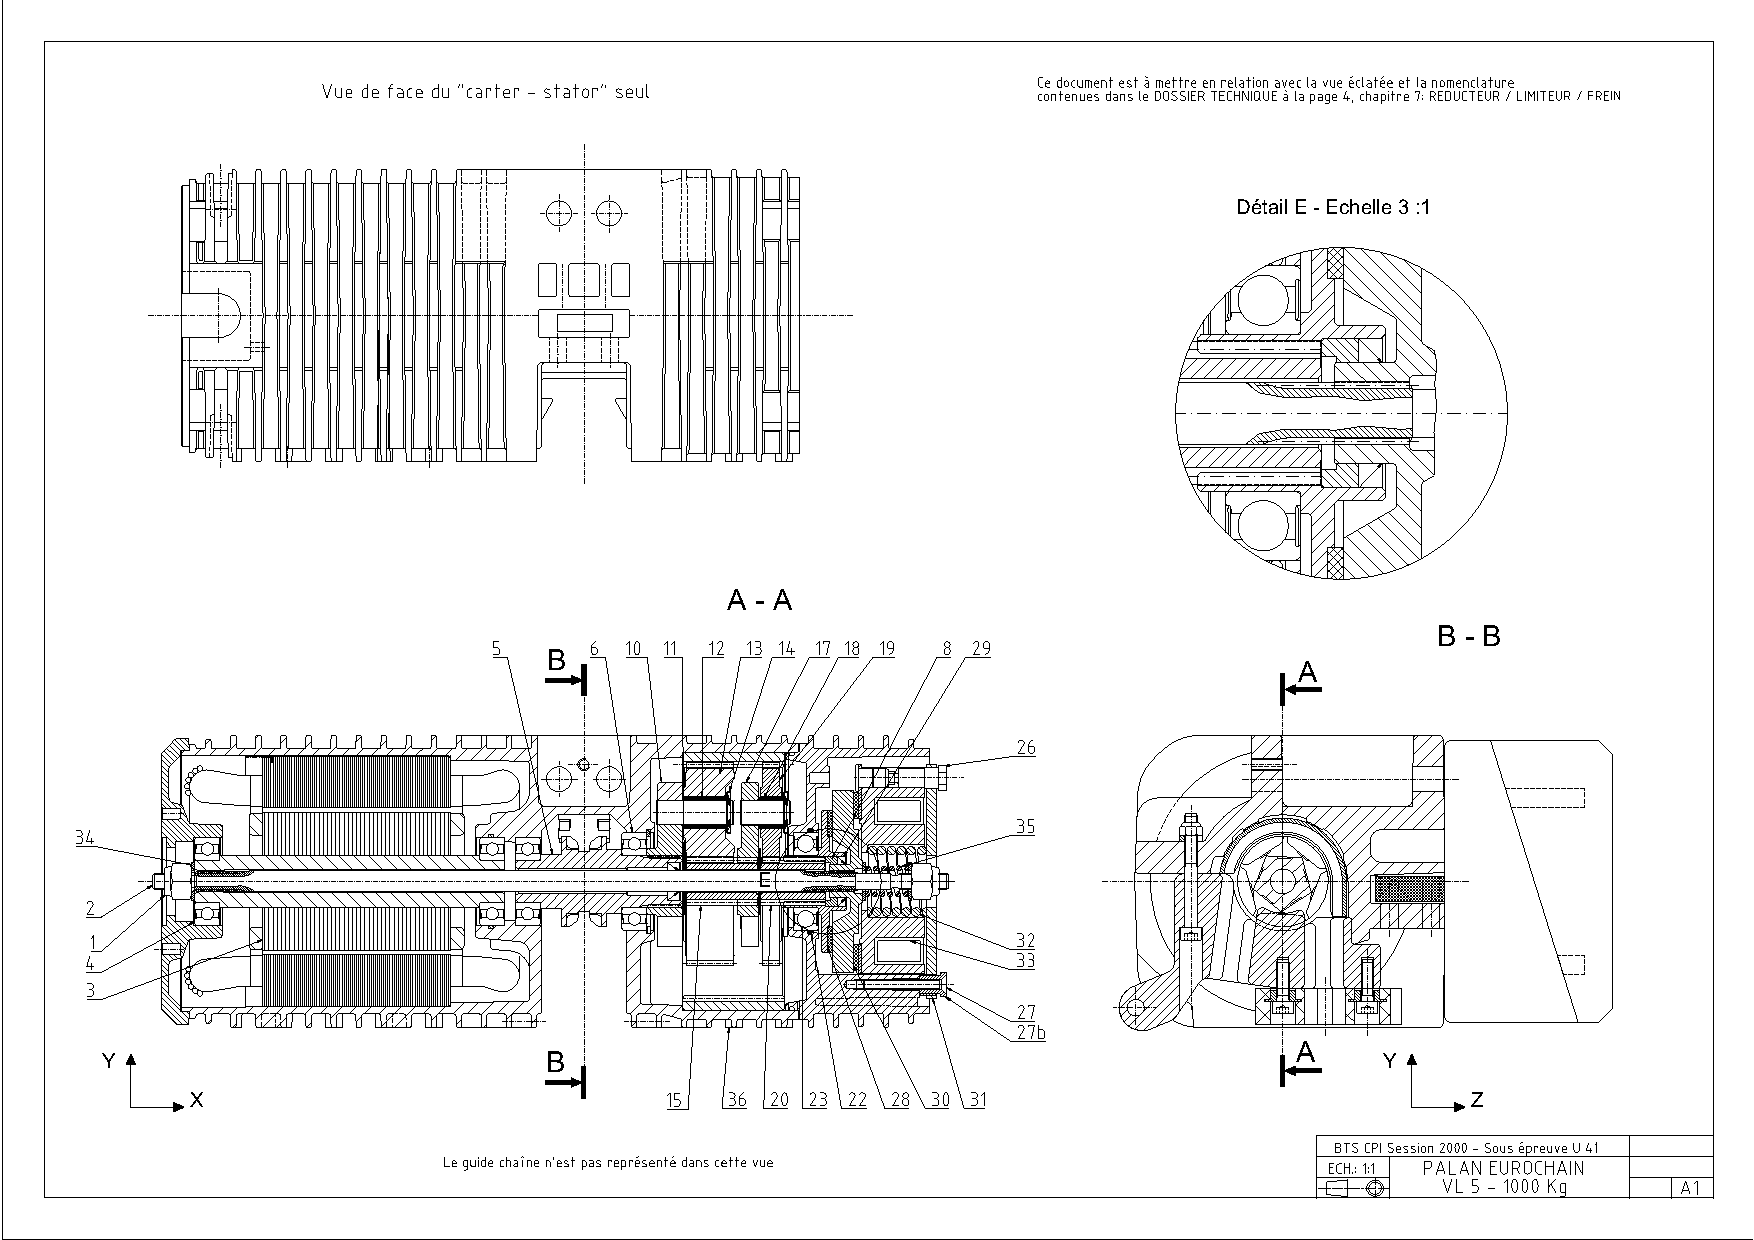
\includepdf[landscape]{img/Palan_Eurochain.pdf}

\newpage

\section{La surfaceuse}

\subsection{Présentation}
\begin{figure}[!h]
\begin{minipage}{0.6\linewidth}
Une surfaceuse est un outil qui permet grâce à la rotation d'un disque rugueux de polir une surface.

La surfaceuse étudiée dans cet exercice est une surfaceuse à béton, elle est alimentée par de l'énergie pneumatique.
\end{minipage}
 \hfill
\begin{minipage}{0.35\linewidth}
 \centering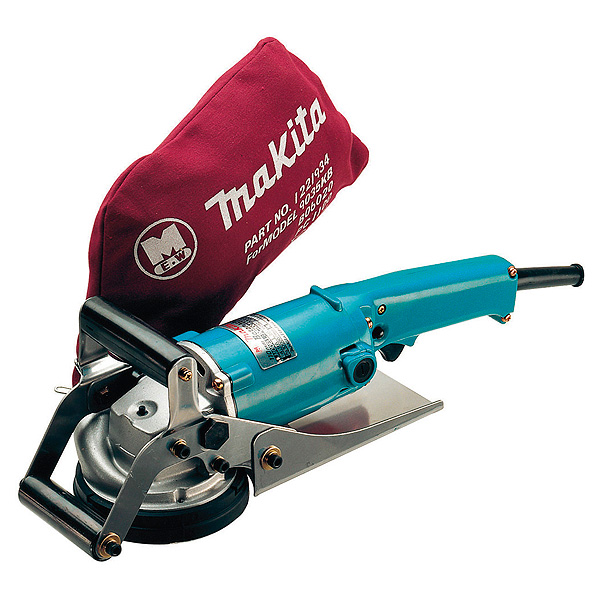
\includegraphics[width=0.7\linewidth]{img/surfaceuse.jpg}
 \caption{Surfaceuse à main}
 \label{fig8}
\end{minipage}
\end{figure}

\subsection{Rapport de réduction}

\paragraph{Question 1:} Déterminer le rapport de réduction du train d'engrenage de cette surfaceuse. Est-il nécessaire de connaître le module des engrenages utilisés?

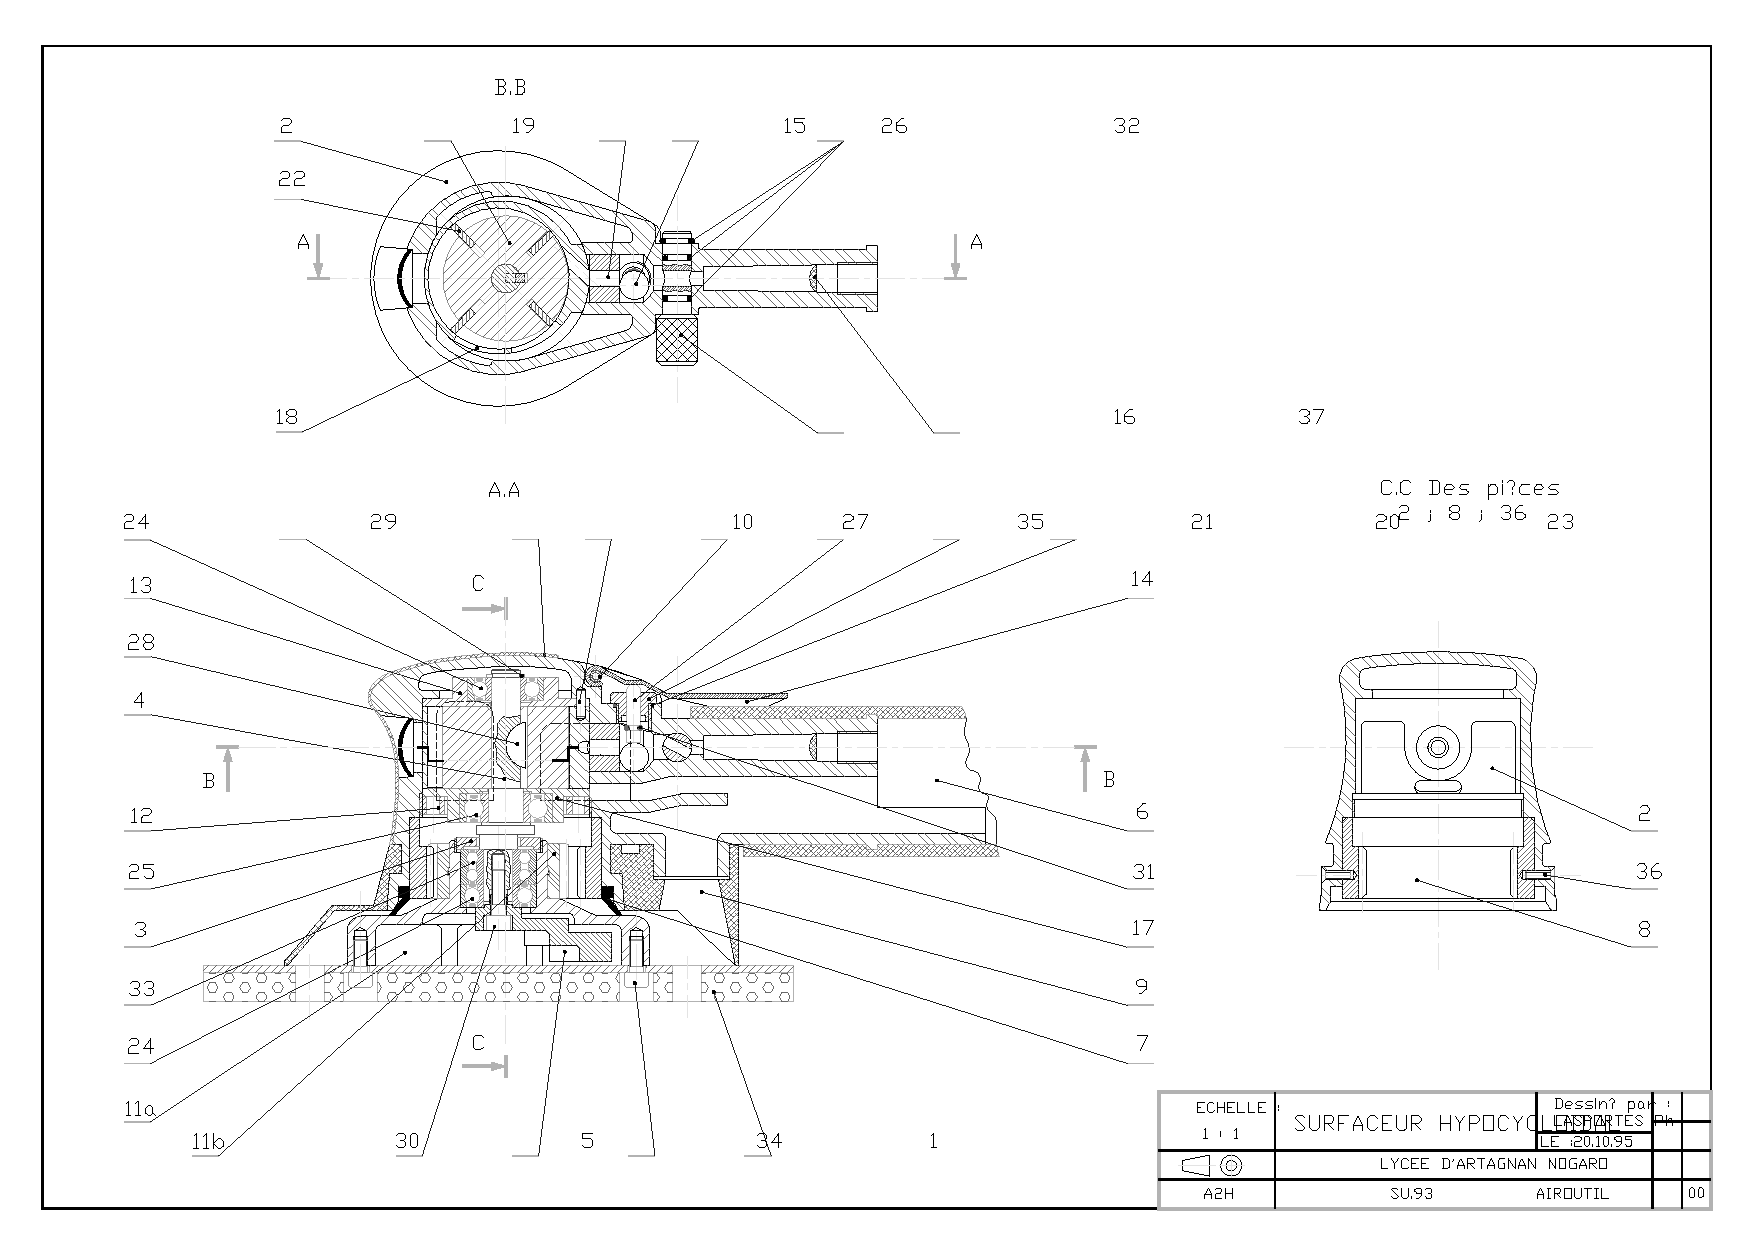
\includepdf[landscape]{img/surfaceuse.pdf}

\newpage

\section{Module REDEX}

\subsection{Présentation}
\begin{figure}[!h]
\begin{minipage}{0.6\linewidth}
La gamme des réducteurs SR est conçue autour d'un train d'engrenages épicycloïdal avec satellites multiples, et permet d'offrir un couple très élevé et une grande gamme de rapports de réduction dans un encombrement limité.
\end{minipage}
 \hfill
\begin{minipage}{0.35\linewidth}
 \centering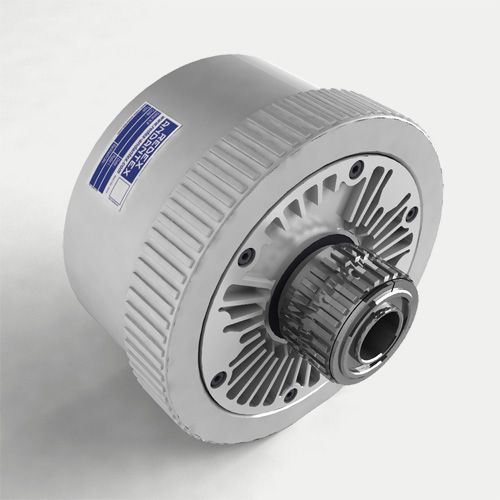
\includegraphics[width=0.7\linewidth]{img/redex.jpg}
 \caption{Module Redex}
 \label{fig9}
\end{minipage}
\end{figure}

\subsection{Rapport de réduction}

\paragraph{Question 1:} Déterminer $\omega_{20}$ pour les cas de figure suivants:

Avec $\omega_{10}=0$ et $\omega_{30}=\omega_e$.

\begin{itemize}
 \item Pour $Z_1=50dents$, $Z_2=50dents$, $Z_{51}=25dents$, $Z_{52}=25dents$,
 \item Pour $Z_1=51dents$, $Z_2=49dents$, $Z_{51}=24dents$, $Z_{52}=26dents$,
 \item Pour $Z_1=52dents$, $Z_2=48dents$, $Z_{51}=23dents$, $Z_{52}=27dents$.
\end{itemize}

\paragraph{Question 2:} Refaire les mêmes calculs avec $\omega_{30}=0$ et $\omega_{10}=\omega_e$.

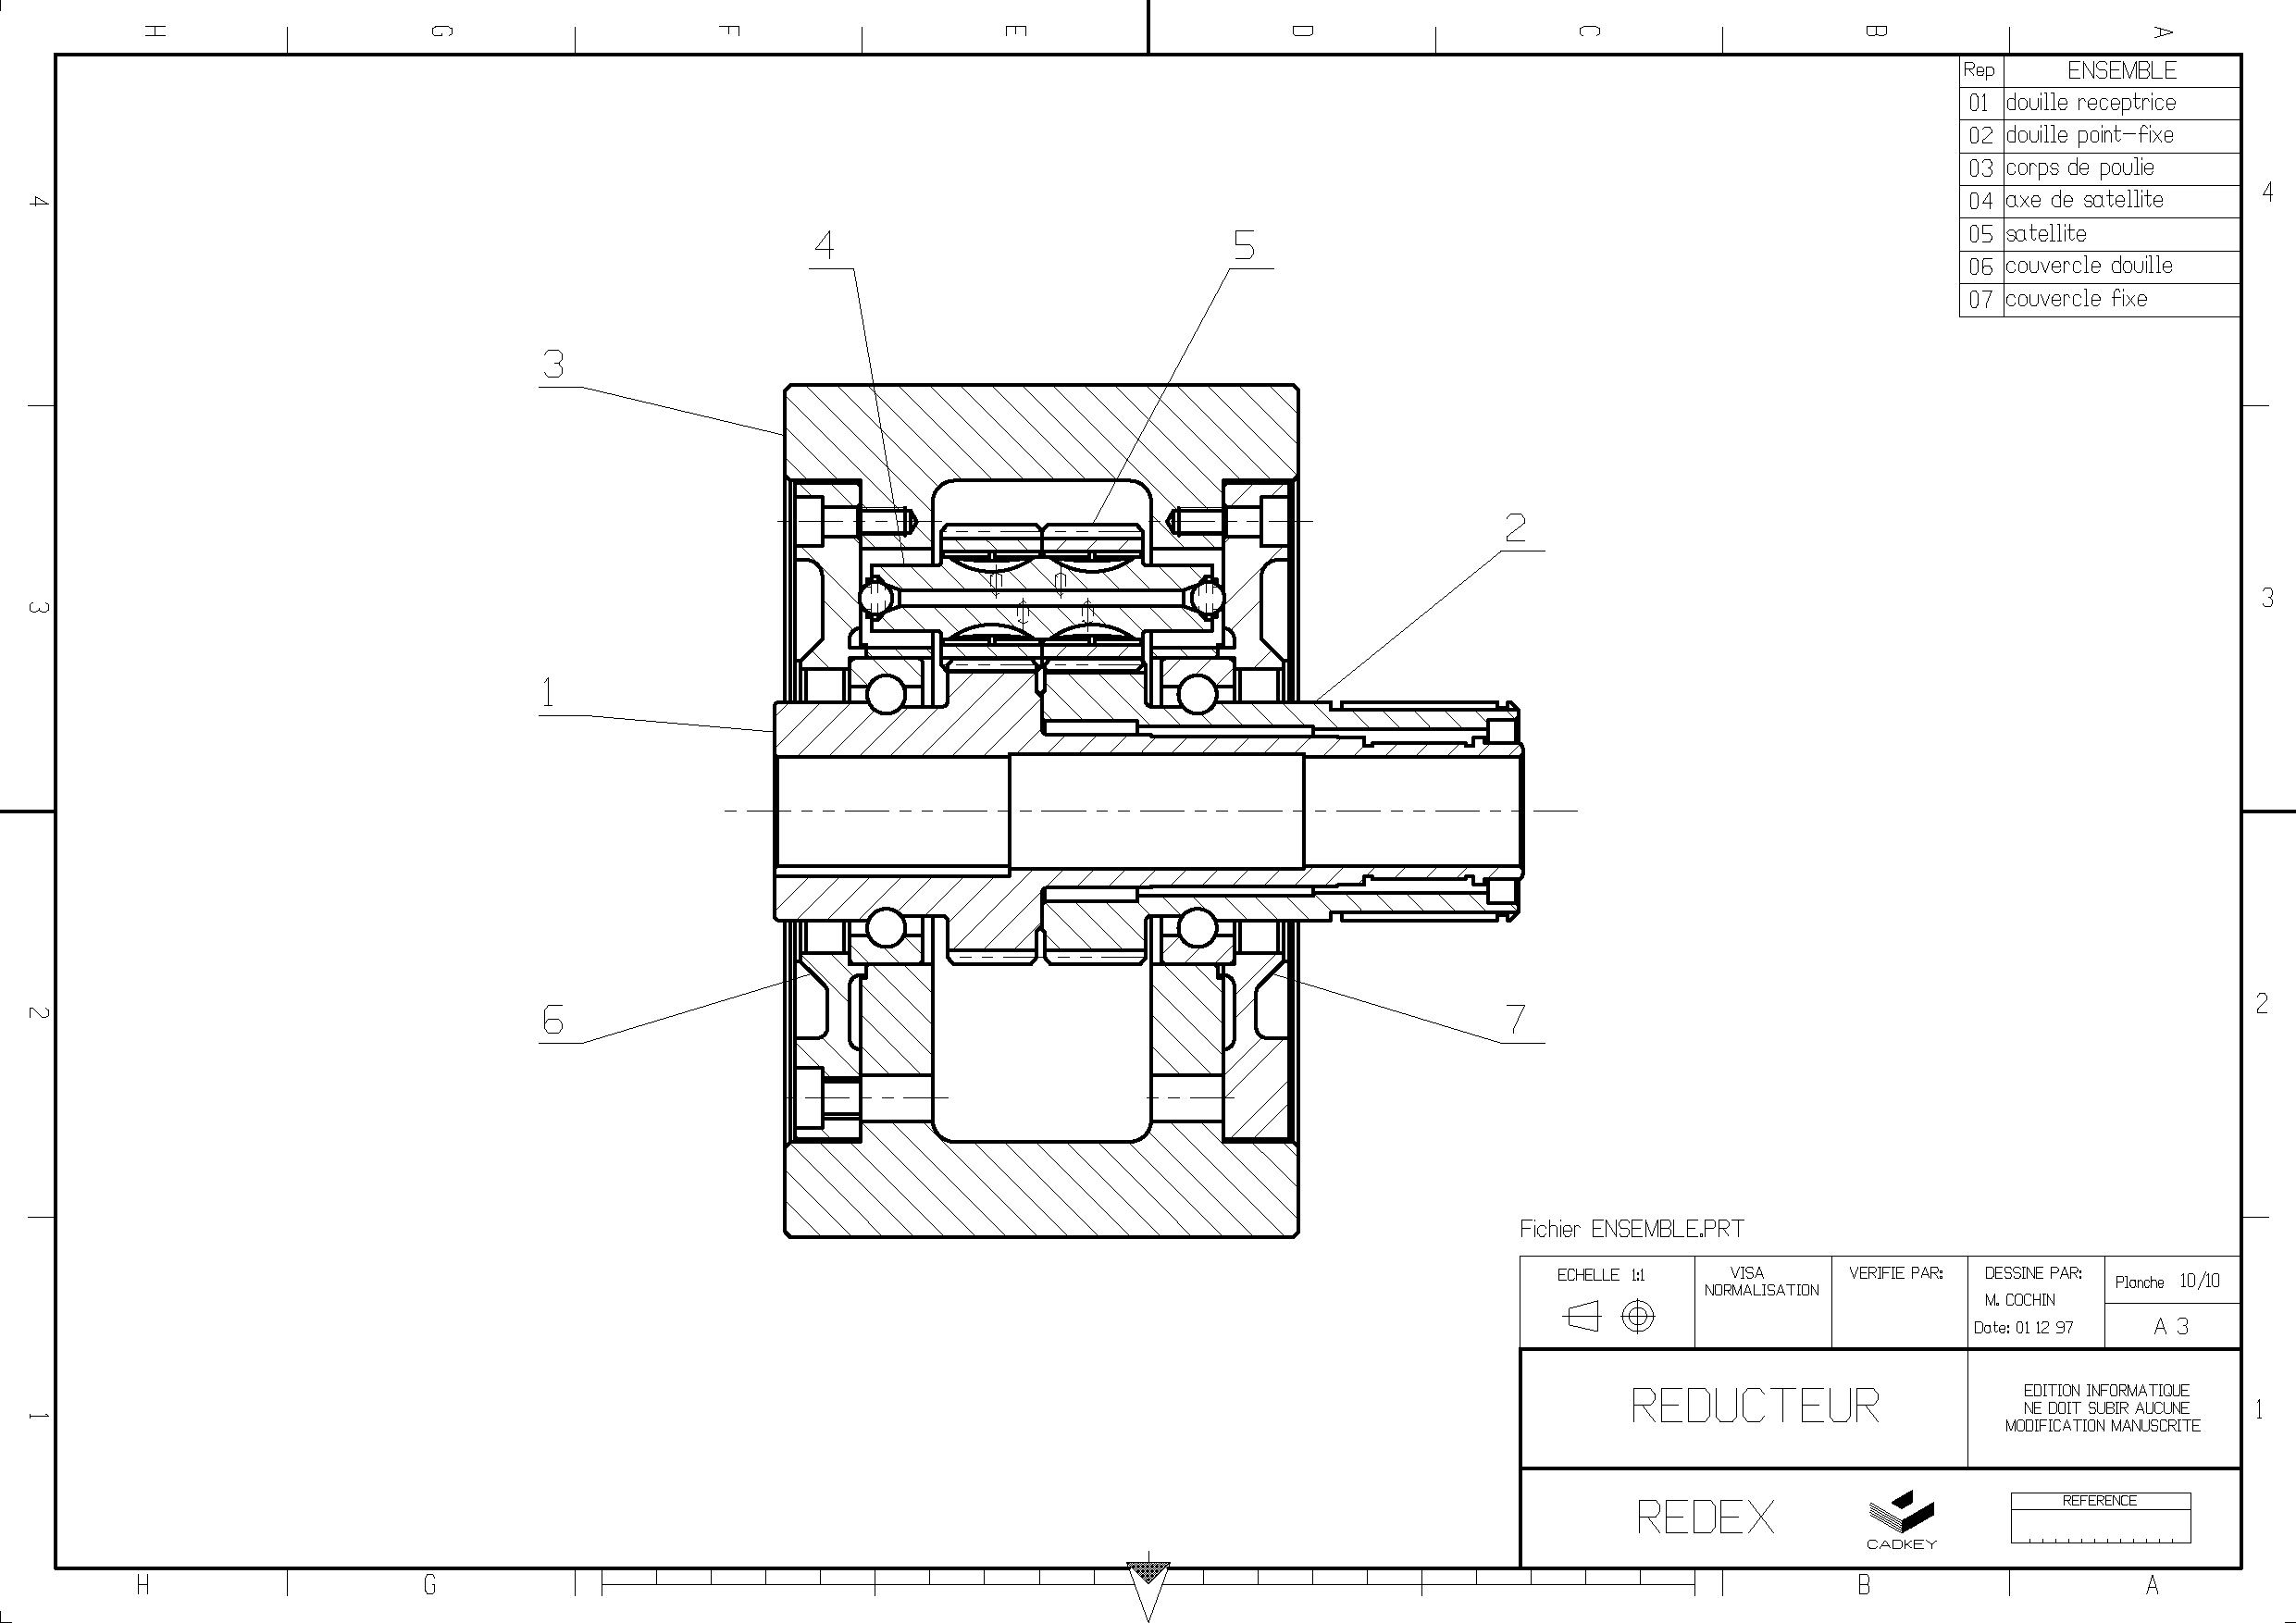
\includepdf[landscape]{img/Module_REDEX.pdf}

\clearpage

\ifdef{\public}{\end{document}}{}

\newpage

\pagestyle{correction}

\section{Correction}

\subsection{Boîte CATEP}

\cor{Boite 1}

\begin{center}
\begin{tabular}{|c|c|c|c||c|}
\hline
100/102 & 1/2 & 101/103 & 1/2 & 1/4\\
\hline
100/102 & 1/2 & 107/104 & 7/5 & 7/10\\
\hline
109/106 & 1 & 101/103 & 1/2 & 1/2\\
\hline
109/106 & 1 & 107/104 & 7/5 & 7/5\\
\hline
108/107 & 5/7 & 101/103 & 1/2 & 5/14\\
\hline
108/107 & 5/7 & 107/104 & 7/5 & 1\\
\hline
\end{tabular}
\end{center}

\begin{enumerate}
 \item 1/4
 \item 5/14
 \item 1/2
 \item 7/10
 \item 1
 \item 7/5
\end{enumerate}

\cor{Boite 2}

\begin{center}
\begin{tabular}{|c|c|}
\hline
209/205 & 1 \\
\hline
-208/207 & -1 \\
\hline
\end{tabular}
\end{center}

\begin{enumerate}
 \item 1
 \item -1
\end{enumerate}

\setcounter{num_cor}{0}
\subsection{Réducteur S.N.T}

\cor{$\omega_r>0$ et $\frac{\omega_r}{\omega_v}=\frac{1}{40}$}

\setcounter{num_cor}{0}
\subsection{Palan Eurochain VL5}

\cor{Le moteur électrique entraîne un train épicycloïdal qui réduit la vitesse de rotation. Le système de frein laisse tourner le palan s'il est alimenté en énergie électrique mais le bloque en cas de coupure de courant pour éviter la chute de la charge. Lorsque le système fonctionne en limiteur, il laisse descendre doucement une charge lourde afin de ne pas endommager le système. Il limite donc le couple au niveau du moteur.}

\newpage

\cor{}

\begin{center}
 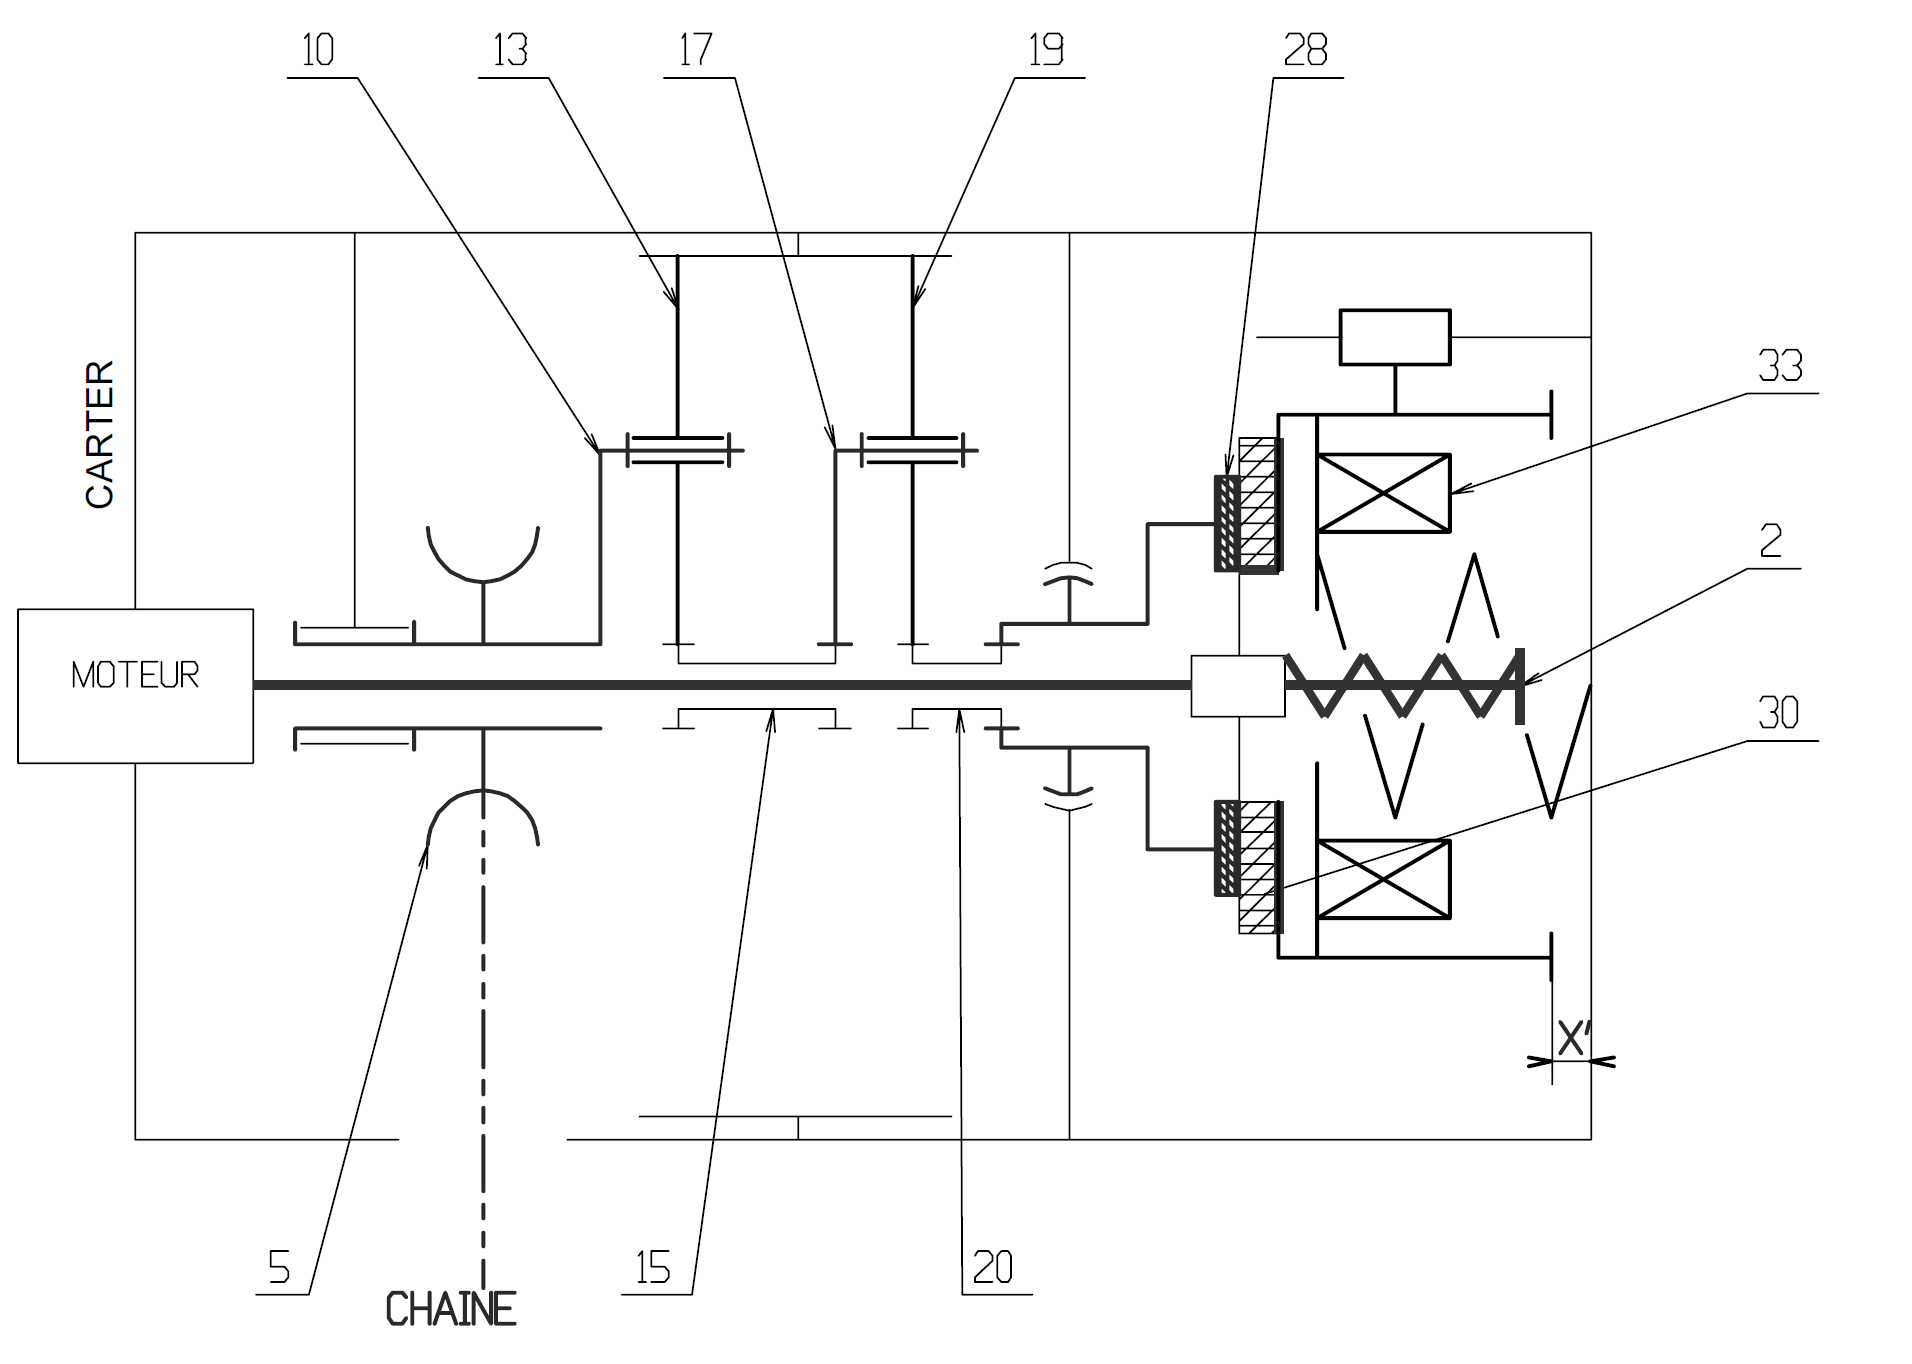
\includegraphics[width=0.8\linewidth]{img/schema_techno}
\end{center}

\cor{Avec 1 train:
$\frac{\omega_c-\omega_{ps}}{\omega_p-\omega_{ps}}=-\frac{Z_p}{Z_c}=-\frac{16}{89}$

Donc $\frac{\omega_{ps}}{\omega_p}=\frac{16}{105}$

Avec 2 trains: $\frac{\omega_s}{\omega_e}=\frac{16}{105}.\frac{16}{105}=\frac{256}{11025}\simeq0,023$
}

\setcounter{num_cor}{0}
\subsection{Surfaceuse}

\cor{Le disque de la surfaceuse est monté sur le satellite. La vitesse d'entrée est celle du porte satellite, la couronne est immobile et il n'y a pas de planétaire.}

\begin{center}
 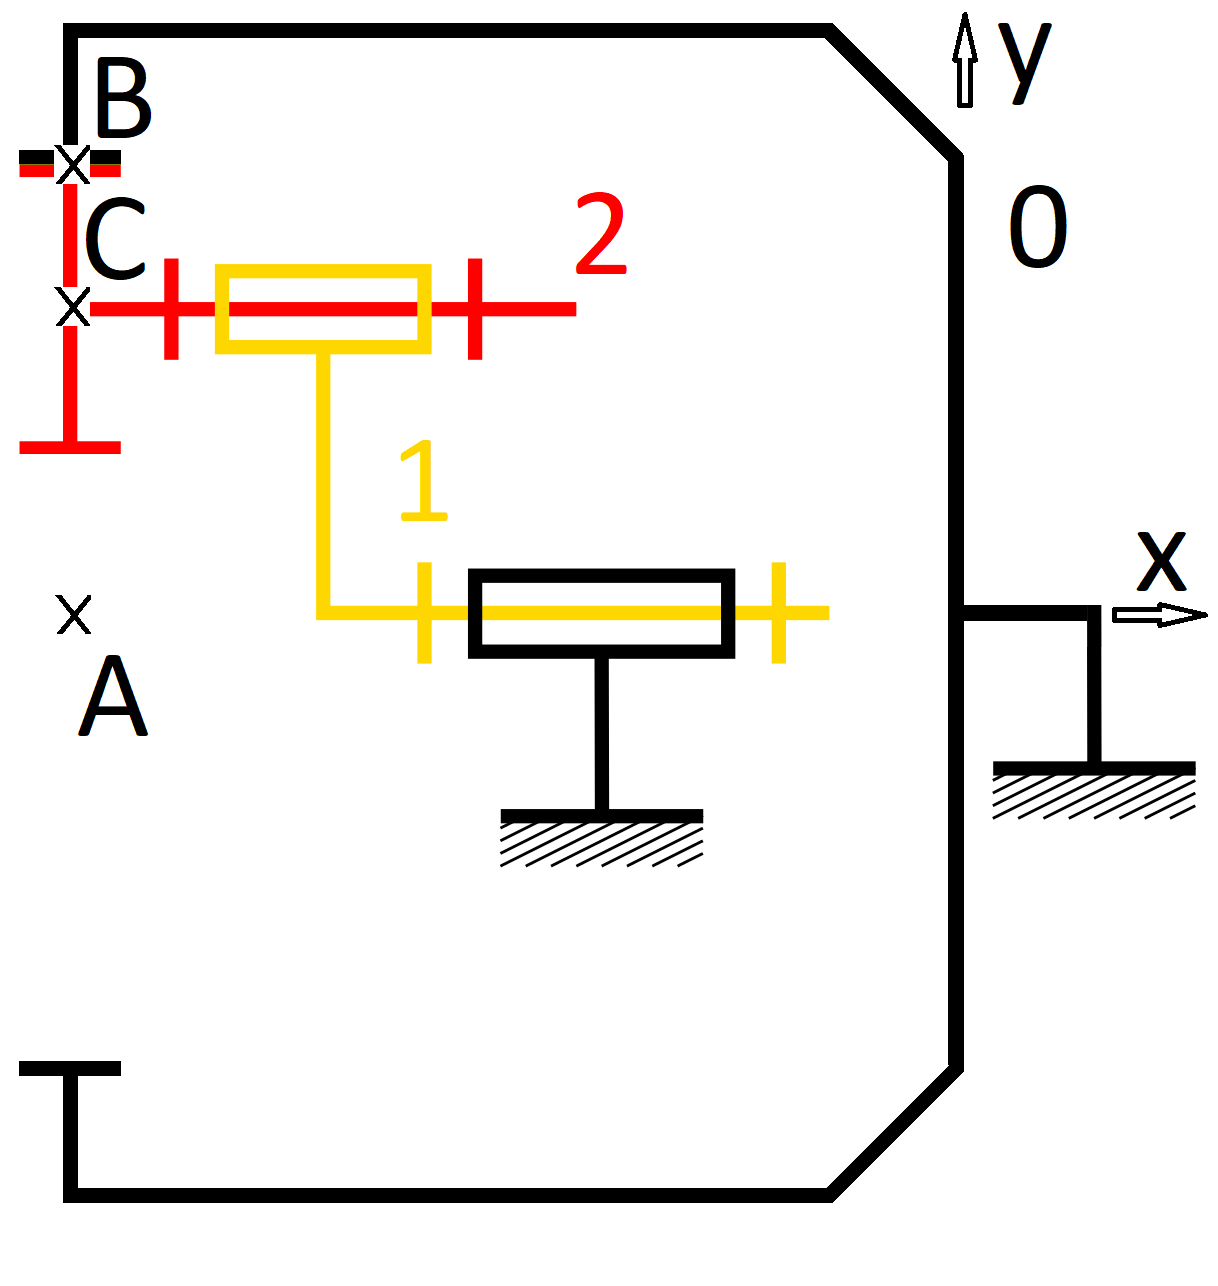
\includegraphics[width=0.6\linewidth]{img/surfaceuse_cin}
\end{center}

$\overrightarrow{V_{A\in1/0}}=\vec{0}$, $\overrightarrow{V_{C\in2/1}}=\vec{0}$, $\overrightarrow{V_{B\in2/0}}=\vec{0}$

$\overrightarrow{V_{B\in2/0}}=\overrightarrow{V_{B\in2/1}}+\overrightarrow{V_{B\in1/0}}$

$\overrightarrow{BC}\wedge\overrightarrow{\Omega_{2/1}}+\overrightarrow{BA}\wedge\overrightarrow{\Omega_{1/0}}=\vec{0}$

$-r.\overrightarrow{y_1}\wedge\omega_{21}.\vec{x}-R.\overrightarrow{y_1}\wedge\omega_{10}.\vec{x}=\vec{0}$

$r.\omega_{21}+R.\omega_{10}=0$

$\frac{\omega_{21}}{\omega_{10}}=-\frac{R}{r}$

Il n'est pas nécessaire de connaître le module.

\setcounter{num_cor}{0}
\subsection{Module REDEX}

$\frac{\omega_{20}-\omega_{30}}{\omega_{10}-\omega_{30}}=\frac{Z_1.Z_{52}}{Z_2.Z_{51}}$

\begin{tabular}{|c|c|c|}
\hline
& $\omega_{10}=0$ & $\omega_{30}=0$ \\
\hline
Cas 1 & $\omega_{20}=0$ & $\omega_{20}=\omega_{10}$ \\
\hline
Cas 2 & $\omega_{20}=-0,13.\omega_e$ & $\omega_{20}=1,13.\omega_e$ \\
\hline
Cas 3 & $\omega_{20}=-0,27.\omega_e$ & $\omega_{20}=1,27.\omega_e$ \\
\hline
\end{tabular}


\end{document}
